\documentclass[submission,copyright,creativecommons]{eptcs}
\providecommand{\event}{SYNT 2018} % Name of the event you are submitting to
\usepackage{breakurl}             % Not needed if you use pdflatex only.
\usepackage{underscore}           % Only needed if you use pdflatex.

\usepackage{booktabs} % For formal tables
\usepackage{amsmath}%
\usepackage{amssymb}
\usepackage{wasysym}%
\usepackage{cleveref}
\usepackage{graphicx}
\usepackage{chngpage}
\usepackage{subcaption}
\usepackage{xcolor}
\usepackage{amsthm}
\usepackage{algorithm}
\usepackage{algorithmic}
\usepackage[normalem]{ulem} % cross line, should be removed later

\title{Warm-Starting Fixed-Point Based Control Synthesis}
\author{Zexiang Liu \qquad\qquad Necmiye Ozay
\institute{EECS\\
University of Michigan\\
Ann Arbor, United States}
\email{zexiang@umich.edu \quad\qquad necmiye@umich.edu}
\and
Nicolas Perrin
\institute{CNRS UMR 7222, ISIR \\
	Sorbonne Universit\'{e} \\
Paris, France}
\email{\quad perrin@isir.upmc.fr  }
}
\def\titlerunning{Warm-Starting Fixed-Point Based Control Synthesis}
\def\authorrunning{Z. Liu, N. Ozay \& N. Perrin}

\theoremstyle{definition}
\newtheorem{example}{Example}
%\newtheorem{proof}{Proof}
\theoremstyle{definition}
\newtheorem{definition}{Definition}
\theoremstyle{remark}
\newtheorem{remark}{Remark}
\theoremstyle{definition}
\newtheorem{assumption}{Assumption}
\theoremstyle{definition}
\newtheorem{problem}{Problem}
\theoremstyle{definition}
\newtheorem{theorem}{Theorem}

\newcommand*{\QEDB}{\hfill\ensuremath{{\blacksquare}}}%

\begin{document}
\maketitle

\begin{abstract}
In this work we propose a patching algorithm to incrementally modify controllers, synthesized to satisfy a temporal logic formula, when some of the control actions become unavailable. The main idea of the proposed algorithm is to ``warm-start" the synthesis process with an existing fixed-point based controller that has a larger action set. 
By exploiting the structure of the fixed-point based controllers, our algorithm avoids repeated computations while synthesizing a controller with restricted action set. Moreover, we show that the algorithm is sound and complete, that is, it provides the same guarantees as synthesizing a controller from scratch with the new action set.    
An example on synthesizing controllers for a simplified walking robot model under ground constraints is used to illustrate the approach. In this application, the ground constraints determine the action set and they might not be known a priori. Therefore it is of interest to quickly modify a controller synthesized for an unconstrained surface, when new constraints are encountered. Our simulations indicate that the proposed approach provides at least an order of magnitude speed-up compared to synthesizing a controller from scratch.
\end{abstract}

\section{INTRODUCTION}
%Paragraph 1: significance of control synthesis. potential applications. control synthesis for augmented finite transition systems. progress groups. 

%What is control synthesis? What is abstraction-based control synthesis? Which type of problems it tries to solve? 

%What's abstraction? What's synthesis?

Control synthesis techniques for discrete systems have been a central topic both for reactive synthesis and discrete-event systems \cite{pnueli1989synthesis,ramadge1987supervisory} with recent results establishing a connection between the two communities \cite{ehlers2017supervisory,schmuckrelation}. These techniques provide a principled means for computing a controller with correctness guarantees for systems that can either be directly modeled as or whose continuous-dynamics can be abstracted as a discrete transition system. Such discrete controllers are ubiquitous in many embedded applications. 

%Paragraph 3: Related work from Livingston.
A key challenge in control synthesis is scalability. The scalability depends both on the size of the discrete transition system and the complexity of the specification, e.g., can be doubly exponential in the length of a general linear temporal logic (LTL) specification \cite{pnueli1989synthesis}. Therefore, some research has focused on identifying fragments of LTL that have favorable complexity (see e.g., \cite{bloem2012synthesis,ehlers2011generalized,wolff2013efficient,Nilsson2017}). Although these fragments lead to tractable problems, the time required for synthesis still prevents it from being applicable on-line, necessitating to consider all possible scenarios at design-time. This motivates the following questions: (i) If controllers are to be synthesized off-line for many different scenarios, and if there is a controller for a specific scenario in hand, can this controller be used to synthesize new controllers efficiently? (ii) can this modification approach be fast enough to enable on-line synthesis if new situations are encountered at run-time? 

The problem of incrementally modifying an existing controller, i.e., ``patching" a controller, as opposed to re-synthesizing from scratch, has been studied for different control synthesis techniques, specifically in the context of robotics applications \cite{Livingston,Livingston2014,wong2014correct}. Livingston et al. \cite{Livingston} study a patching method for two player games with the specifications given by the GR(1) fragment of LTL and the control strategies synthesized by a $ \mu $-calculus based method. Assuming that changes in system and environment only break an existing controller locally, they re-synthesize a controller only for the affected nodes and replace the broken part with the new one. When ``localness" assumption or estimation of the affected states fails, the performance of this method could degrade to the case that does synthesis from scratch. This method is also extended to handle changes in the specification such as addition of new goal regions \cite{Livingston2014}. Wong et al. \cite{wong2014correct} also consider GR(1) specifications with corresponding symbolic controller synthesis techniques and develop recovery mechanisms when the environment assumptions become invalid during execution. 

This paper also considers the problem of patching controllers. Different from the existing literature mentioned above, we work with synthesis problems where there exists an explicit transition system to be controlled and the modification required is due to some of the control actions becoming unavailable. The loss of control actions is relevant in the case of actuator faults and also in the context of stabilizing a hopping robot on a constrained surface, as described later. Another difference is the class of specifications considered: the LTL fragment we use includes persistence requirements, which are not expressible within the GR(1) fragment, and is amenable to fixed-point based control synthesis techniques operating directly on the transition system (see e.g., \cite{wolff2013efficient,Nilsson2017}). Our main contribution is to propose a novel \emph{controller implementation}, a data structure consisting of a partially ordered set of controllers corresponding to simple fixed-points in the synthesis algorithm,  that captures all the information required for modification when some of the actions become unavailable. We then present patching techniques using this data structure that modifies it appropriately to compute the new controller. The proposed patching techniques are in a sense similar to warm-starting techniques in optimization, where an existing solution (not too far away from the expected new solution) is used to initialize an optimization algorithm. Similarly, we use an existing controller to initialize the synthesis algorithm for finding a controller for the new problem. 

%, but they consider a different type of LTL fragment $ GR(1) $ and control strategies synthesized by $ \mu $-calculus based method. Assuming that changes in system and environment only break an existing controller locally, they re-synthesize a controller only for the affected nodes and replace the broken part with the new one. When ``localness" assumption or estimation of the affected states fails, the performance of this method could degrade to the case that does synthesis from scratch.


%Paragraph 2: summary of our method

%Control implementation (the data structure and how it is utilized).

%Paragraph 3: Related work from Livingston.
%How are works related to our paper? What's the problem they try t o solve? What's the difference with ours? What's our advantages?

%We dive into the structure of existing controllers, remove the unnecessary parts for the new action profile and then take it as an intermediate result to warm-start the synthesis process, until it converges to the new controller.


%(there two other papers)

% Paragraph 4: Motivation
We demonstrate the proposed approach on a push recovery example for a 1D hopping robot. The potential control actions for the robot are the feasible foot placements. However, if there are ground constraints, e.g., holes, obstacles, on which the robot is not allowed to step, the available action set reduces. Such constraints might not be available a priori, hence, it is of interest to design many controllers for different sets of ground constraints. In addition, if one wants to use 1D push recovery controllers to navigate a 2D surface with constraints, it is again possible (albeit some conservatism) to consider a large number of 1D ground constraint profiles and corresponding family of 1D controllers for the 2D navigation task. Our results for this example show that up to an order of magnitude speed-up can be achieved if the controllers for constrained surface are generated by patching the controller for the unconstrained surface.  

%Motivation: Talk more about the hoping robot. Mention actuator faults (losing and actuator)

%Paragraph 5: 

The paper is organized as follows: In Section \ref{sec:pre}, we give the problem statement and the background knowledge about fixed-point based control synthesis. Section \ref{sec:method} presents the main algorithm that warm-start a control synthesis from an existing controller, and the proof of soundness and completeness. We use a simple running example in Sections \ref{sec:pre} and \ref{sec:example} to illustrate how the method works before presenting an example on control synthesis for a hopping robot in Section \ref{sec:example} that shows the time efficiency and potential applicability of our method.

\section{PRELIMINARIES}
\label{sec:pre}
\subsection{Notation}

For two sets $ A $ and $ B $, the set difference is denoted by $ A-B $. A function or a map $ F: C\rightarrow D $ {\color{purple} corresponds to  the set} $ \{(c,F(c)):c\in C, F(c)\in D \} $.{\color{teal}A list $ \mathcal{V}=[x_1,...,x_n] $ is a totally ordered set, where $ \mathcal{V}(i) $ refers to its $ i $th-order element. To assign $ x_i $ to be the $ i $th element in	 $ \mathcal{V} $ is written as $ \mathcal{V}(i) = x_i $.} {\color{purple} Not sure it is really useful to define functions or maps here, the terms are barely used in the rest of the document (function x4, map x1)} 

\subsection{Augmented Finite Transition Systems}

\begin{definition}
	An \textbf{augmented finite transition system} (AFTS) \cite{Nilsson2017} is a tuple $ T = (Q,U,\rightarrow_T, G,AP,h_Q) $, where $ Q $ is a set of states, $U$ is a set of actions (control inputs), $ \rightarrow_T\in Q\times U \times Q $ is {\color{purple} is a transition relation} between states under specific actions, $ G: 2^U\rightarrow 2^{2^Q} $ {\color{teal}maps a set of actions to a set of progress groups\footnotemark under that action set }, $ AP $ is a finite set of atomic propositions, and $ h_Q: Q\rightarrow 2^{AP} $ is a labeling function, which maps states to the set of atomic propositions they preserve {\color{purple} verify}. \footnotetext{\color{purple} %Maybe a few words on the progress group maps, which is a non-standard notion:	
	A set $G \in G(D)$ is called a \emph{progress group under the action set $D$} , and it is related to the following semantic notion: the system cannot remain indefinitely within
		$G$ by exclusively choosing actions from $U$. This restricts the behaviors allowed by the transition relation. (see \cite{Nilsson2017,Sun2014,Liu2014})}
\end{definition}

\begin{definition}
	A \textbf{control strategy} for an AFTS is a partial function $ \mu:~(Q\times U)^*\times Q\rightarrow 2^U $ which maps the history of state-action pairs and the current state to a set of actions.
\end{definition}

\subsection{Linear Temporal Logic}

Linear Temporal Logic (LTL) can be utilized to describe the desired behaviors of an AFTS system. It has logic operators (negation $ \neg $, conjunction $ \wedge $, disjunction $ \vee $), and temporal operators (next $ \bigcirc $, always $ \Square $, eventually $ \Diamond $ and until $ \mathbf{\ U\ }$).

%{\color{blue} use grammar to define LTL, cite Baier and Katoen}
%The LTL formula over a finite set of atomic propositions $ AP $ can be either: 
%\begin{itemize}
%	\item $ True $
%	\item $ p\in AP $ 
%	\item $ \neg \phi , \phi \vee \psi, \bigcirc \phi $ and $ \phi \mathbf{\ U\ } \psi $ for LTL formulas $ \phi $ and $ \psi $. 
%\end{itemize}

{\color{teal}\emph{ Syntax of LTL} \cite{baier2008principles}: The LTL formula over a finite set of atomic propositions $ AP $ can be formed according to the grammar:}
\begin{displaymath}
	\phi := True\ \vert\ p\ \vert\ \phi_1 \vee \phi_2\ \vert\ \neg \phi\ \vert\ \bigcirc \phi\ \vert\ \phi_1 \mathbf{U}\phi_2
\end{displaymath}
%{\color{blue}what is the numbering vi, v, etc. below?} 
where $ p\in AP $, $ \phi_1 $ and $ \phi_2 $ are also LTL formulas. The other operators can be derived as follows: $ \phi_1 \wedge \phi_2 = \neg (\neg \phi_1 \vee \neg \phi_2) $, $ \phi_1 \implies \phi_2 = \neg \phi_1 \vee \phi_2 $, $ \Diamond \phi = True \mathbf{\ U\ } \phi $, $ \Square \phi = \neg \Diamond \neg \phi $.

{\color{teal}\emph{Semantics of LTL} \cite{Nilsson2017}:} An $\omega$-word is an infinite sequence in $ 2^{AP}$.  The satisfaction of an LTL specification $ \phi $ by an $\omega$-word $ w = w(0)w(1)w(2)\dots $, written as $ (w,i) \models \phi $, is defined inductively as follows:
\begin{itemize}
	\item For $ \phi = p \in AP $, $ (w,i)\models p $ iff $ p\in w(i) $ 
	\item $ (w,i)\models \neg \phi $ iff $ (w,i)\not\models \phi $
	\item $ (w,i)\models  \phi_1 \vee \phi_2 $ iff $ (w,i)\models \phi_1 $ or $ (w,i)\models \phi_2 $
	\item $ (w,i) \models \bigcirc \phi $ iff $ (w,i+1) \models \phi $
	\item $ (w,i)\models \phi_1 \mathbf{\ U\ } \phi_2 $ iff $\exists j\geq i  $ s.t. $ (w,j)\models \phi_2 $ and $ (w,k)\models \phi_1, \forall k\in [i,j) $
\end{itemize} 

An $\omega$-word $ w $ satisfies $ \phi $ if and only if $ (w,0)\models \phi $, written as $ w \models \phi $. 

Given a trajectory of an AFTS $ s = \{s(n)\}_{n=0}^{\infty} $, the \textit{$\omega$-words} of y is $ h_Q(s) =  \{h_Q(s(n))\}_{n=0}^{\infty} $, where $ h_Q $ is the labeling function of the AFTS.  Given a LTL specification $ \phi $, we say that $ s\models \phi $ if and only if $ h_Q(s) \models \phi $.

\subsection{Control Synthesis and Fixed-Point Operators}
\label{sec: cont_syn}
\iffalse
The procedure of abstraction-based control synthesis is as follows: 

\begin{itemize}
	\item[i] For a continuous or discrete system, find its over-approximate {\color{purple} finite} AFTS abstraction. For instance, given the dynamics of a robot system with {\color{purple} a bounded} state space, we can discretize its state space into {\color{purple} a finite set of nodes} and compute the transitions among them over-approximately,  {\color{purple} leading to an abstraction of the system}.
	\item[ii] Determine the LTL specification which describes the desired system behaviors. For example, given a mobile robot and a region $ A $ in the state space, the specification $ \Square A $ {\color{purple} would be used to force the robot to remain in $A$ indefinitely.}. 
	\item[iii] Based on the abstraction and LTL specification, search {\color{purple} a} winning set and control strategy such that {\color{purple} any trajectory starting from a state of the winning set and respecting the control strategy always verifies the given specification.} the system trajectories which start from any state in the winning set and follow the control strategy will satisfy the given specification.
\end{itemize}
\fi

%{\color{blue}I just noticed G is used for progress group. Maybe we can use R (for recurrence) if it is not used for something else}

The specification considered in this work is of the form:
\begin{align}
\phi = \Square A \wedge \Diamond \Square B \wedge \left( \bigwedge_{i\in I} \Square \Diamond R^i\right)\label{phi}
\end{align}
{\color{purple} for subsets $A$, $B$, $R^i \subseteq Q$ defining atomic propositions. Such specifications can express properties of \emph{invariance} ($\Square A$), \emph{persistence} ($\Diamond \Square B$) and \emph{reccurence}} 

{\color{blue}Maybe we should say a few words on how this fragment differs from GR(1) and others}

%{\color{blue} Maybe we should say "the winning set" since it is unique when defined to be the largest.} {\color{purple} Yes, when it is stated that we consider the largest, we should use "the" I agree (but in the previous version it wasn't mentioned I think).}
\begin{definition}
	The \textbf{winning set} of the specification $ \phi $ over an AFTS $ T = (Q, U, \rightarrow_T, G, AP, h_Q) $, written as $ W_{\phi} $, is the largest subset of $ Q $ such that if the system $ T $ is initially in $ W_{\phi} $, specification can be enforced.
\end{definition}

\begin{definition}
	A \textbf{simple controller} for a winning set $ W $ over an AFTS is a function $ \mathcal{C}: $ W $ \rightarrow 2^U $, i.e. a memoryless controller. A simple controller maps the current state to a set of actions under which the specification in the winning set remains guaranteed.
	\label{def:simp}
\end{definition}

Given $\widehat{W} \subseteq W $, a simple controller $ \mathcal{C} $ \textbf{restricted to} $ \widehat{W} $ means that the domain of $ \mathcal{C} $ is restricted to $\widehat{W}$.

\begin{definition}
	For the AFTS $ T=\{Q,U,\rightarrow_T,G,AP,h_Q\} $, a \textbf{controller} $ \mathcal{C} $ for a winning set $ \text{Win}^T(\phi) $ is a tuple $ (\mathcal{V},\mathcal{K},x) $, where $ \mathcal{V} $ is a list of subsets of $ Q $, $ \mathcal{K} $ is a list of controllers or simple controllers, i.e. so-called sub-controllers of $ \mathcal{C} $, and $ x $ is an internal variable that saves the index of sub-controllers called last time.
	\label{def:cont}
\end{definition}
 
 Overall, a controller is a tree structure with controllers at each node and simple controllers at the leaf nodes. The list $\mathcal{K}$ for each controller (node) denotes the children of that controller in the tree.



{\color{purple} Winning sets and controllers} for specifications in the form of \eqref{phi} are computed iteratively via the following fixed-point based algorithm {\color{purple} (see \cite{Nilsson2017})}.

%\begin{remark}
%	The definition of controller defines the implementation of a control strategy obtained by fixed-point operators discussed in the following. For \eqref{win_phi}, \eqref{win_interm}, \eqref{win_until} and \eqref{win_inv}, the number of sub-controllers in each controller is proportional to the number of iterations when the corresponding fixed-point operator converges. Simple controllers are smallest elements in a controller, i.e. the ones given by \eqref{eqn:pre} and \eqref{win_inv}. 
%\end{remark}

\begin{align}
& [V_{\infty},\mathcal{C}] =\  \text{Win}_{\exists, \forall}^{T,U}\left(\Square A \wedge \Diamond \Square B \wedge \left( \bigwedge_{i\in I} \Square \Diamond R^i\right)\right)\\
=&\begin{cases}V_{\text{inv}} = \text{\text{Win}}^{T,U}_{\exists, \forall} ((A\mathbf{U}\emptyset)\vee \Square (A\wedge \Diamond Q))\\
\text{Restrict~ synthesis~ to~ }V_{\text{inv}}\\
V_0 = \emptyset,\ \mathcal{V}=\{\},\ \mathcal{K} = \{\}\\
while\ V_{k+1} \not= V_k:\\
\ \ \ \ Z_{k+1} = \text{Pre}_{\exists,\forall}^{T,U} (V_k) \bigcup \text{PGPre}_{\exists,\forall}^{T,U} (V_k, Q)\\
\ \ \ \ [V_{k+1}, \mathcal{C}_{k+1}]=\text{Win}_{\exists,\forall}^{T} ((B \mathbf{\ U\ }Z_{k+1}) \vee \Square (B\wedge ( \bigwedge_{i\in I}\Diamond R^i))\\
\ \ \ \ \mathcal{V}(k+1)=V_{k+1},\ \mathcal{K}(k+1) = \mathcal{C}_{k+1}\\
V_{\infty} = V_k,\ \mathcal{C}=(\mathcal{V},\mathcal{K},x)
\end{cases}\label{win_phi}
\end{align}

The winning set {\color{purple} that results from} \eqref{win_phi} is {\color{purple} equal to} $ V_{\infty} $, i.e. {\color{purple} the limit of the expanding sequence $V_k$}. $ \mathcal{C} $ is the controller corresponding to the winning set $ V_{\infty} $. 

The building blocks of the above algorithm are the following fixed-point operators. Each operator corresponds to a type of LTL formula used in \eqref{win_phi}. (Note that when a fixed-point operator appears as part of a formula, it only refers to its first output, i.e. the winning set.)

\begin{align}
&[W_{\infty},\mathcal{C}]= \ \text{Win}_{\exists,\forall}^{T,U}((B\mathbf{\ U\ }Z)\vee \Square (B\wedge(\bigwedge_{i\in I}\Diamond R^i)) )\\
=&\begin{cases}
W_0 = Q,\ \mathcal{V}=\{\},\ \mathcal{K}=\{\}\\
while\ W_{k+1}\not= W_k:\\
\ \ \ \ Z_{k+1}^i = Z\cup (B\cap R^i\cap \text{Pre}_{\exists, \forall}^{T,U}(W_k))\\
\ \ \ \ [X^i, \mathcal{C}^i]= \text{Win}_{\exists,\forall}^{T,U} (B\mathbf{\ U\ }Z_{k+1}^i), \forall i \in I\\
\ \ \ \ W_{k+1} = \bigcap_{i\in I} X^i\\
\mathcal{V}(1)=W_k,\ \mathcal{V}(i+1) = B\cap R^i,\ 
\mathcal{K}(i) = \mathcal{C}^i, \forall i\in I\\
W_{\infty} = W_k,\ \mathcal{C} = (\mathcal{V},\mathcal{K},x)
\end{cases}\label{win_interm}
\end{align}
\begin{align}
&[X_{\infty},\mathcal{C}]= \text{Win}_{\exists,\forall}^{T,U} (B\mathbf{\ U\ }Z)\\
=&\begin{cases}
X_0 = \emptyset,\ \mathcal{V}=\{\},\ \mathcal{K}=\{\}\\
while\ X_{k+1}\not= X_k\\
\ \ \ \ [V^1_k,C^1_k]=
\text{Pre}_{\exists,\forall}^{T,U}(X_k)\\
\ \ \ \  [V^2_k,C^2_k]=\text{PGPre}_{\exists,\forall}^{T,U}(Z\cup(B\cap V^1_k),B)\\
\ \ \ \ X_{k+1} =Z\cup (B\cap V^1_k)\cup V^2_k\\
\ \ \ \ \mathcal{V}(2k+1)=V^1_k, \mathcal{V}(2k+2)=V^2_k\\
\ \ \ \ \mathcal{K}(2k+1)=C^1_k,\ \mathcal{K}(2k+2)=C^2_k\\
X_{\infty}=X_k,\ \mathcal{C} = (\mathcal{V},\mathcal{K},x)
\end{cases}\label{win_until}
\end{align}
\begin{align}
&[Z_{\infty},\mathcal{C}]=\text{PGPre}_{\exists,\forall}^{T,U} (Z,B)\\
=&\begin{cases}
Z_{\infty} = Z,\ \mathcal{V} = \{\},\ \mathcal{K}=\{\}, k = 1\\
for\ U\in 2^U:\\
\ \ for\ G\in G(U):\\
\ \ \ \ \ \  [V_k,\mathcal{C}_k]=Inv_{\exists}^{U,G}(Z_{\infty},B)\\
\ \ \ \ \ \ Z_{\infty} = Z_{\infty} \cup V_k\\
\ \ \ \ \ \ \mathcal{V}(k)=V_k,\ \mathcal{K}(k)=\mathcal{C}_k,\ k++\\
\mathcal{C} = (\mathcal{V},\mathcal{K},x)
\end{cases}\label{win_pgpre}
\end{align}
\begin{align}
&[W,\mathcal{C}]=\text{Pre}_{\exists,\forall}^{T,U}(V)\\
=&\begin{cases}
W = \{q_1\in Q: \exists (u\in U) \forall (q_2\ s.t.\ (q_1, u, q_2) \in \rightarrow_T), q_2\in V\}\\
D(q)=\{u\in U: \forall (q_2\ s.t.\ (q,u,q_2)),\ q_2\in V\}\\
\mathcal{C}=\{(q,D(q)):q\in Q, D(q)\not=\emptyset\}
\end{cases}\label{eqn:pre}\\
&[Y_{\infty},\mathcal{C}]=\text{Inv}_{\exists}^{D,G}(Z,B)\\
=&\begin{cases}Y_0 = (G\cap B) - Z\\
while\ Y_{k+1}\not=Y_k:\\
\ \ \ \ Y_{k+1} = Y_k\cap \text{Pre}_{\exists,\forall}^{T,D}(Y_k\cup Z)\\
[-,\mathcal{C}] = Pre^{T,D}_{\exists,\forall}(Y_k\cup Z)\\
Y_{\infty} = Y_k,\ \mathcal{C}\ restricted\ to\ Y_{\infty}
\end{cases} \label{win_inv}
\end{align}

The winning sets {\color{purple} resulting from} \eqref{win_interm}, \eqref{win_until}, \eqref{win_inv} are $ W_{\infty} $, $ X_{\infty} $ and $ Y_{\infty} $. {\color{purple} $\text{Pre}_{\exists,\forall}^{T,U}$ is a one-step reachability operator, and $\text{Inv}_{\exists}^{U,G}(Z,B)$ computes $Y_\infty \subseteq (G\cap B) - Z$ from where the state can be controlled (with actions in $U$) to either remain inside $Y_\infty$ or reach $Z$, but because $G$ is a progress group under $U$, remaining indefinitely in $G$ is impossible and therefore $Z$ is
	eventually reached, which is why $Y_\infty$ is a winning set for $B\mathbf{\ U\ }Z$.}

%The control strategy enforcing the specification in the winning set $ W_{\phi} $ can be extracted in the meantime when executing the fixed-point operators \cite{Nilsson2017}. 
%{\color{purple} The control strategy enforcing the specification in $ W_{\phi} $  can be extracted while computing the limits $ V_{\infty} $, $ W_{\infty} $, $ X_{\infty} $ and $ Y_{\infty} $. As stated in \cite{Nilsson2017}, 
%all the fixed points are ultimately defined in terms of $\text{Pre}_{\exists,\forall}^{T,U}$, so it is enough to extract control strategies during calls to this operator and map the results into higher-level fixed points together with internal variables that control a hierarchy of partial reachability objectives.}

\begin{definition} \textbf{Execution of controllers}:
In the execution time, a controller $ \mathcal{C}=(\mathcal{V},\mathcal{K},x) $ acts as a function that maps the current state in $ Q $ to a set of feasible actions in $ U $, for the AFTS $ T = (Q,U,\rightarrow_T, G,AP,h_Q)$. Given the current state $ s $, the output $ \mathcal{C}(s) $ is determined in two steps:
\begin{itemize}
	\item[(i)] update the internal variable $ x $ of $ \mathcal{C} $: 
	\begin{itemize}
		\item 	if $ \mathcal{C} $ is returned by \eqref{win_phi},\eqref{win_until},\eqref{win_inv}:
		\begin{displaymath}
		x^+ =	\begin{cases}
		\text{arg}\min_{y\leq x}\{s\in \mathcal{V}(y)\},\ \ if\ x\not=0\\
		\text{arg}\min_{y}\{s\in \mathcal{V}(y)\},\ \ otherwise
		\end{cases}
		\end{displaymath}
		\item  if $ \mathcal{C} $ is returned by \eqref{win_interm}:
		\begin{displaymath}
		x^+ = \begin{cases}
		x\mod\vert\mathcal{K}\vert + 1,\ \ if\ s\in \mathcal{V}(x+1)\\
		x,\ otherwise
		\end{cases}
		\end{displaymath}
	\end{itemize}
	where $ x^+ $ refers to the value of internal variable $ x $ after update.

	\item[(ii)] Return the output of the $ x^+ $th sub-controller in $ \mathcal{K} $ with input $ s $, i.e.
	\begin{displaymath}
	\mathcal{C}(s) = \mathcal{K}(x^+)(s)
	\end{displaymath}
\end{itemize}
	
	In the execution of $ \mathcal{K}(x^+)(s) $, the process above would be repeated and then a sub-controller of $ \mathcal{K}(x^+) $ would be executed. Thus it's a recursive process that doesn't end until a simple controller is reached.
	The set of feasible actions will be returned by that simple controller. For those sub-controllers not called in this execution, their internal variables keeps unchanged.
	

	%Assume the current state is $ s_t $. Each time a controller is called with input $ s_t $, the controller updates its internal variable according to $ s_t $, the winning sets of sub-controllers and the current value of internal variable. Then, the sub-controller indexed by the new value of internal variable would be called with $ s_t $ as input. Repeat the above procedure inductively until a simple controller is reached, which returns the set of feasible actions for $ s_t $. \label{ref:cont}
	\label{def:exec}
\end{definition}
{\color{purple} For me there is a problem of clarity with the definition of controllers, especially with the internal variable. I think we should explain in the definition roughly what happens when a call to the controller is made: if I understood well the memory variable changes according to some finite state automaton (we could say that and say that an example of how it works precisely is given below. But if the controller indeed needs the transition graph it is not just a tuple, we should add the transitions of the internal variables in the definition. Or am I missing something? Also overall the way this transition graph is constructed from the fixed-point operators (at least an intuition of it) is missing.}


\begin{figure}
	\centering
	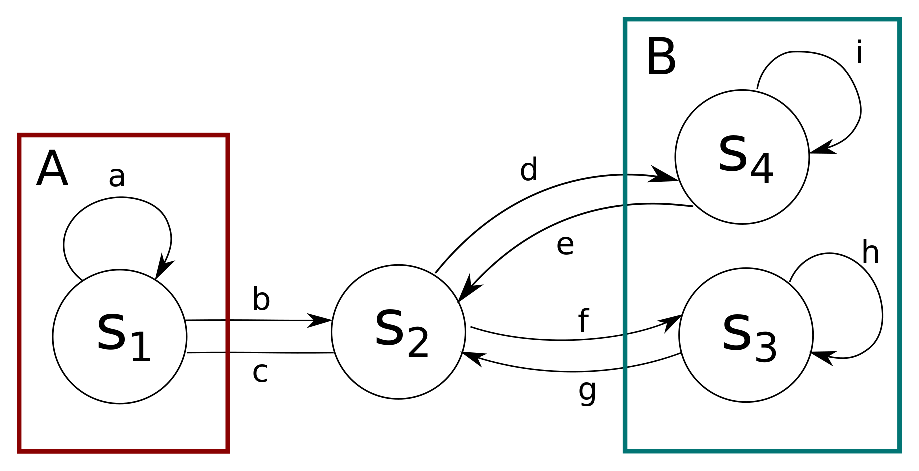
\includegraphics[width=0.7\linewidth]{pic/eg1}
	\caption{A simple finite transition system with state space $\{s1,s2,s3,s4\}$ and action space $\{a-h\}$, used to illustrate how the controller works. Atomic propositions are $ A =\{s_1\} $ and $ B=\{s_3, s_4\} $.}
	\label{fig:eg1}
\end{figure}

\begin{example}
	For a simple transition system shown in Figure \ref{fig:eg1}, given the specification $ \phi = \Square \Diamond A \wedge \Square \Diamond B $, the outputs of \eqref{win_phi} are winning set $ W= \{s_1,s_2,s_3,s_4\}$, and controller $ \mathcal{C} = (W,\{\mathcal{C}^0_1\}, x = 1) $, where the sub-controllers are:
	
	$ \mathcal{C}^0_1 = (\{W,\{s_1\},\{s_3,s_4\}\},\{\mathcal{C}^1_1, \mathcal{C}^1_2\}, x^0_1 ) $; 
	
	$ \mathcal{C}^1_1 = (\{\{s_1,s_2\},W,W \},\{\mathcal{C}^{2,0}_i\}_{i=1}^3,x^1_1)$;
	
	$ \mathcal{C}^1_2 = (\{\{s_2,s_3,s_4\},W,W \}\{\mathcal{C}^{2,1}_i\}_{i=1}^{3},x^1_2 )$, $ \mathcal{C}^{2,0}_1 = \{(s_1,\{a\}),(s_2,\{c\})\} $;
	
	$ \mathcal{C}^{2,0}_2 = \{(s_1,\{a,b\}),(s_2,\{c\}),(s_3,\{g\}),(s_4,\{e\})\} $;
	
	$ \mathcal{C}^{2,0}_3 = \{(s_1,\{a,b\}),(s_2,\{c,d,f\}),(s_3,\{g,h\}),(s_4,\{e,i\})\} $; 
	
	$ \mathcal{C}^{2,1}_1 = \{(s_2,\{d,f\}),(s_3,\{h\}),(s_4,i)\} $; 
	
	$ \mathcal{C}^{2,1}_2 = \{(s_1,\{b\}),(s_2,\{d,f\}), (s_3,\{g,h\}), (s_4,\{e,i\})\} $;
	
	$ \mathcal{C}^{2,1}_3 = \{(s_1,\{a,b\}),(s_2,\{c,d,f\}),(s_3,\{g,h\}),(s_4,\{e,i\})\} $.
	
%	\begin{figure}
%		\centering
%		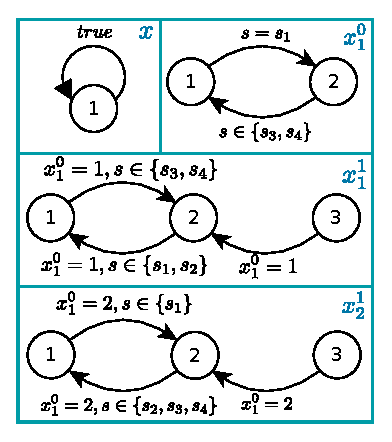
\includegraphics[width=0.7\linewidth]{pic/xupdate}
%		\caption{ Update $ x$ first, and then $ x^0 $, and lastly $ x_0^1 $ and $x^1_1 $. $ s $ is the current state. The transition condition is labeled on the edge. Self loop exists (ignored on the graph): one variable keeps unchanged if no condition satisfies.}
%		\label{fig:xupdate}
%	\end{figure}
	
	$ \mathcal{C} $, $ \mathcal{C}_1^0 $ and $ \mathcal{C}_i^1 $ are returned by \eqref{win_phi}, \eqref{win_interm} and \eqref{win_until}. $ \mathcal{C}_i^{2,k} $ are simple controllers returned by \eqref{eqn:pre}. Each time $ \mathcal{C} $ is called, $ (x,x^0_1,x^1_1,x^1_2) $ is updated according to Definition \ref{def:exec}, and one of the simple controllers is called to determine the set of feasible control inputs. %is determined by $ \mathcal{C}^{2,k}_{x^1_{k}} (s)$ (if $ x^0 = k  $).
	
	For example, initialize the internal variables to be $ (1,1,1,1) $. Let's start from $ s_1 $ and run $ \mathcal{C}(s_1) $: The updated internal variables would be $ (1,2,1,2) $, after $ \mathcal{C}(s_1), \mathcal{C}^0_1(s_1)$, $ \mathcal{C}^1_2(s_1) $ and $ \mathcal{C}^{2,1}_2(s_1) $ are called recursively. The set of feasible actions is $ \{b\}= \mathcal{C}^{2,1}_2(s_1) $. Under action $ b $, the system in Figure \ref{fig:eg1} transits to $ s_2 $. Now run $ \mathcal{C}(s_2) $. The internal variable would be updated to $ (1,2,1,1) $. The set of feasible actions is$ \{d,f\}=\mathcal{C}^{2,1}_1(s_2) $. Let's keep doing this and always take the first action in the output of $ \mathcal{C} $ at each execution. The trajectory under control of $\mathcal{C} $ would be $ s_1,s_2,s_4,s_2,s_1,...$, where the sequence of actions is $ b,d,e,c,... $. The trajectory visits $ A $ and $ B $ in turn, satisfying the given specification.
	
	%\footnote{Define $ x_{total}: = (x,x^0,x^1_0,x^1_1) $. Each $ x_{total} $ locates a simple controller, i.g. $ x_{total}  = (0,1,0,5)$  gives that $ C_0^0\rightarrow C^1_1\rightarrow C^2_5 $. The evolution of $ x_{total} $ in the example above is $ (0,0,0,0), (0,1,0,5),(0,1,0,4), (0,0,1,4), (0,0,0,4)... $.}
\end{example}

{\color{blue} don't use b.w., s,t, use between, such that. in general, it is better writing practice to avoid abbreviations as much as possible}

\subsection{Problem Statement}

In this section, we formally define the problem of interest. {\color{blue}it is usually a good idea to start with telling what you want to do in the section so that the user is prepared.}

{\color{purple} Somewhere we should give the main steps of the solution also. I think one thing that would be important is to state clearly what can and cannot change in the structure of the controller when $U$ is modified. I guess it is not only a change of the transitions, like in the example, since in some cases the number of steps to convergence can be modified. But then what exactly remains invariant? Only the "depth" of the controller? }

\begin{problem}
	Given an AFTS $ T = (Q,U,\rightarrow_T,G,AP,h_Q) $, a LTL specification $ \phi = \Square A \wedge \Diamond \Square B \wedge \left( \bigvee_{i\in I} \Square \Diamond R^i\right) $, the winning set $ W_{\phi} $ and controller $ \mathcal{C}_{\phi} $, if a set of actions $ U_d\subseteq U $ in $ T $ is unavailable, find the new winning set and a controller based on $ W_{\phi} $ and $ \mathcal{C}_{\phi} $.
\end{problem}


\section{PATCHING METHOD}
\label{sec:method}

Before presenting the patching methods, we state a property of controller implementations that roughly shows that the controllers contain all the relevant information needed for patching. We start with a definition of strategy containment.

\begin{definition}
	For two control strategies $ \mu_1 $ and $ \mu_2 $ with winning set $ W_1 $ and $ W_2 $, we say $ \mu_2 $ contains $ \mu_1$, denoted as $ \mu_{1} \subseteq \mu_{2}$, if $ \mu_{1} (\{(s_i,a_i)\}_{i=1}^{n-1}, s_n) $ is a subset of $ \mu_{2}(\{(s_i,a_i)\}_{i=1}^{n-1}, s_n) $, for all feasible $ n $ and all transition trajectories $ q =(s_1,a_1),(s_2,a_2),...,(s_{n-1},a_{n-1}) $ satisfying $ s_1\in W_{1} $, $ a_k \in \mu_{1} (\{(s_i,a_i)\}_{i=1}^{k-1}, s_k) $.
\end{definition}

Consider an AFTS $ T = (Q,U,\rightarrow_T,G,AP,h_Q) $ and {\color{blue} an} LTL specification $ \phi = \Square A \wedge \Diamond \Square B \wedge \left( \bigvee_{i\in I} \Square \Diamond G^i\right) $. Compute its winning set \eqref{win_phi} and the winning control strategy $ \mu_{\phi} $ (or controller $ \mathcal{C}_{\phi} $) via fixed-point operators. Now disable some actions $ U_d \subseteq U$, i.e. getting a new AFTS $ \widehat{T} = (Q,U-U_d,\rightarrow_T,G,AP,h_Q) $ and re-compute the winning set and control strategy, denoted by $ \widehat{W}_{\phi} $ and $ \widehat{\mu}_{\phi} $ (or controller $ \widehat{\mathcal{C}}_{\phi} $), via the same fixed-point operator. Then, we have the following.



\begin{theorem}
	For $ W_{\phi}, \mu_{\phi}, \widehat{W}_{\phi}, \widehat{\mu}_{\phi} $ defined above, we have $ \widehat{W}_{\phi} \subseteq W_{\phi}  $ and $ \widehat{\mu}_{\phi} \subseteq \mu_{\phi}$\label{thm: 1}.
\end{theorem}

\begin{proof}
	(i) For any state $ s\in \widehat{W}_{\phi} $, if the system $ \widehat{T} $ starting from $ s $ could be controlled under an infinite sequence of actions and satisfy the specification, so is $ T $, since $ T $ can apply exactly the same sequence of actions and get the same trajectory. Hence $ s\in W_{\phi} $, for \eqref{win_phi} is sound and complete (See Lemma 13 in \cite{Nilsson2017}). Therefore $ \widehat{W}_{\phi}\subseteq W_{\phi} $. (ii) any control strategy in $ \widehat{T} $ works in $ T $ by construction, which implies $ \widehat{\mu}_{\phi} \subseteq \mu_{\phi}$.
\end{proof}

If $ C_{\phi} $ is implemented to contain all the possible control strategies, Theorem \ref{thm: 1} says that $ \mathcal{C}_{\phi} $ should contain all the information of $ \widehat{\mathcal{C}}_{\phi} $, which implies there is a possibility to obtain $ \widehat{\mathcal{C}}_{\phi} $ by modifying the existing controller.


%From the perspective of implementation, a controller $ \mathcal{C}=(\mathcal{V},\mathcal{K},x) $ is a data structure that organizes simple controllers in a hierarchy way. The partially ordered sets $ \mathcal{V} $  and internal variable are only used during execution. So the basic step for patching a controller is to modify its simple controllers, which are discussed in Section \ref{sec:patching_simple}. 

\subsection{Patching Simple Controllers}
\label{sec:patching_simple}
\begin{definition}
	Given a simple controller $ \mathcal{C} $ over an AFTS $T = (Q,U,\rightarrow_T, G,AP,h_Q) $, a \textbf{finite transition system} (FTS) corresponding to $ \mathcal{C} $ is $T(\mathcal{C}) = (Q_C, U_C, \rightarrow_{T(\mathcal{C})})$, where $ Q_C $ is the set of states that appear in $ \rightarrow_{T(\mathcal{C})} $, $ U_C=\{u: u\in \mathcal{C}(s), \forall s\in W\} $, $ \rightarrow_{T(\mathcal{C})} =\{(s_1,u,s_2)\in \rightarrow_T: s_1\in W,s_2\in Q, u\in \mathcal{C}(s_1)\} $. \label{def:T_C}
\end{definition}

\begin{remark}
	By Definition \ref{def:T_C}, $ T(\mathcal{C}) $ can be easily constructed from the simple controller $ \mathcal{C} $ and the AFTS $ T $. Conversely, $ \mathcal{C} $ can be constructed from $ T(\mathcal{C}) $ by $ \mathcal{C} = \{(s,D(s)):s\in W,D(s)\not=\emptyset\} $, where $ D(s)=\{u:(s,u,s_2)\in \rightarrow_{T(\mathcal{C})}\} $.
\end{remark}
Due to the easy conversion between  $ \mathcal{C} $ and $ T(\mathcal{C}) $, we can modify a simple controller $ \mathcal{C} $ by modifying its corresponding FTS $ T(\mathcal{C}) $ and then converting $ T(\mathcal{C}) $ to $ \mathcal{C} $, with the advantages that $ T(\mathcal{C}) $ contains the necessary transition information, which $ \mathcal{C} $ doesn't have, and is easier to manipulate. 

Assume the AFTS $ T = (Q,U,\rightarrow_T, G, AP, h_Q) $ is the abstraction of the system that needs to be controlled. Assume that $ T(\mathcal{C})=(Q_{\mathcal{C}}, U_{\mathcal{C}},\rightarrow_{T(\mathcal{C})})$ is a transition system corresponding to a simple controller $ \mathcal{C} $. 

Firstly let's define several operation to manipulate the finite transition system $ T(\mathcal{C}) $:

\emph{transitions removing}: given $ E = \{(s_1,a,s_2): s_1,s_2\in Q_{\mathcal{C}}, a\in U_{\mathcal{C}}\} $, remove all transitions in $ E $ from $ T(\mathcal{C}) $ i.e. replace $ \rightarrow_{T(\mathcal{C})} $ with $\rightarrow_{T(\mathcal{C})} - E$, written as 
\begin{displaymath}
	T(\mathcal{C})\backslash E 
\end{displaymath}

There are three variations of this operation:
\begin{itemize}
	\item $ T(\mathcal{C}) \backslash (E,*) \equiv T(\mathcal{C})\backslash \{(s_1,a,s_2)\in \rightarrow_{T(\mathcal{C})}: (s_1,a)\in E)\}$, where $ E \subseteq Q_{\mathcal{C}}\times U_{\mathcal{C}} $.
	\item $ T(\mathcal{C}) \backslash (*,U_d,*) \equiv T(\mathcal{C})\backslash \{(s_1,a,s_2)\in \rightarrow_{T(\mathcal{C})}: a\in U_d \}$, where $ U_d\subseteq U_{\mathcal{C}} $.
	\item $ T(\mathcal{C}) \backslash (Q_d,*,*)\equiv T(\mathcal{C})\backslash \{ (s_1,a,s_2)\in \rightarrow_{T(\mathcal{C})}: s_1\in Q_d \}$, where $ Q_d \subseteq Q_{\mathcal{C}} $ 
\end{itemize}

\emph{transition adding}: given $ E \subseteq Q \times U \times Q$, replace $ \rightarrow_{T(\mathcal{C})} $ with $ \rightarrow_{T(\mathcal{C})}\cup E $, denoted for simplicity by
\begin{displaymath}
T(\mathcal{C})\cup E
\end{displaymath}

Note that since $ E \subseteq Q\times U\times Q $, $ E $ may contain states and actions which do not exists in $ Q_{\mathcal{C}}\subseteq Q $ and $ U_{\mathcal{C}}\subseteq U $. Then just assume that $ Q_{\mathcal{C}} $ and $ U_{\mathcal{C}} $ will enlarge automatically, which is easy to implement in code.

\emph{null node seeking}: return the set $\{s_1\in Q_{T(\mathcal{C})}: \exists (s_1,a,s_2)\in \rightarrow_{T(\mathcal{C})},\forall a\in U_{T(\mathcal{C})}, \forall s_2 \in Q_{T(\mathcal{C})}\} $, i.e. all the nodes whose out-degree is zero, written as
\begin{displaymath}
Vac(T(\mathcal{C}))
\end{displaymath}

\emph{state-action pre}: return the set $ \{(s_1,a): (s_1,a,s_2)\in \rightarrow_{T(\mathcal{C})}, s_2\in S_2\} $, i.e. all the edges pointing into nodes in $ S_2 $, written as
\begin{displaymath}
\widehat{Pre}^{T(\mathcal{C}),U}_{\exists,\exists}(S_2)
\end{displaymath}

Now we are ready to modify simple controllers returned by \eqref{eqn:pre} and \eqref{win_inv}:

Assume that  $ W $ and $ \mathcal{C} $ are the winning set and controller returned by $ \text{Pre}_{\exists,\forall}^{T, U}(V) $. 

Given $ \widehat{V}= V-\Delta V $ and $ \widehat{U} = U-U_d $, we want to modify $ W $ and $ \mathcal{C} $ to be the winning set and controller of $ \text{Pre}_{\exists,\forall}^{T,\widehat{U}}(\widehat{V}) $.  The patching operator is:

\begin{align}
&[\widehat{W},\widehat{\mathcal{C}}]=\overline{\text{Pre}}_{\exists,\forall}^{T, U}(\mathcal{C},\Delta V,U_d)\\
=&\begin{cases} 
T_{0} = T(\mathcal{C})\backslash (*,U_d,*)\\
E =  \widehat{Pre}^{T_0,U-U_d}_{\exists,\exists}(\Delta V)\\
T(\widehat{\mathcal{C}}) = T_{0}\backslash E\\
\widehat{W} = \{s_1: \exists u, \exists s_2 s.t. (s_1,u, s_2)\in \rightarrow_{T(\widehat{\mathcal{C}})} \}
\end{cases}\label{patch_pre}
\end{align}
where $ \widehat{\mathcal{C}} $ is converted from $ T(\widehat{\mathcal{C}}) $. $ \widehat{W} $ and $ \widehat{\mathcal{C}} $ will be equal to the outputs of $ \text{Pre}_{\exists,\forall}^{T,\widehat{U}}(\widehat{V}) $.

\begin{proof}
	Let's assume that $ \text{Pre}_{\exists,\forall}^{T,\widehat{U}}(\widehat{V}) $ returns $ W_t $ and $ \mathcal{C}_t $. It's enough to show that $ T(\widehat{\mathcal{C}})= T(\mathcal{C}_t)$, i.e. $ \rightarrow_{T(\widehat{\mathcal{C}})} = \rightarrow_{T(\mathcal{C}_t)} $. 
	
	By \eqref{eqn:pre} and Definition \ref{def:T_C}, it's obvious that $ \rightarrow_{T(\mathcal{C}_t)} \subseteq \rightarrow_{T(\mathcal{C})}$ for $ \widehat{V}\subseteq V $ and $ \widehat{U}\subseteq U $. The set of transitions $ S = (*,U_d,*)\cup E $ is only related to states in $ \Delta V $ or actions in $ U_d $, so $\rightarrow_{T(\mathcal{C}_t)}$ and $ S $ are disjoint. $ \rightarrow_{T(\widehat{\mathcal{C}})}= \rightarrow_{T(\mathcal{C})}-S$. Thus $ \rightarrow_{T(\mathcal{C}_t)}\subseteq \rightarrow_{T(\widehat{\mathcal{C}})}$ 
	
	By \eqref{patch_pre}, transitions in $ T(\widehat{\mathcal{C}}) $ can only take actions in $ \widehat{U} $ and transit to states in $ \widehat{V} $, which implies that $ \rightarrow_{T(\widehat{\mathcal{C}})}\subseteq \rightarrow_{T(\mathcal{C}_t)} $.  
\end{proof}

Next, $ Y $ and $ \mathcal{C} $ assume that  the winning set and controller resulting from $ \text{Inv}_{\exists}^{D,G}(Z,B) $. Assume that the set of unavailable actions is $ U_d $. If $ D\cap U_d \not= \emptyset$, the winning set would be empty by definition of progress group (see\cite{Nilsson2017}). Given that $ \widehat{Z} \subseteq Z $ and $ D\cap U_d=\emptyset $, we want to modify $ W $ and $ \mathcal{C} $ to be the winning set and controller for $ \text{Inv}_{\exists}^{D,G}(\widehat{Z}, B) $. The patching operator is

\begin{align}
&[\widehat{Y},\widehat{\mathcal{C}}]=\overline{Inv}_{\exists}^{D,G}(Y,\mathcal{C},Z,\widehat{Z}) \\
=&\begin{cases}
Y_0 = Y\cup (\Delta Z\cap G \cap B)\\
\Delta Y_0 = Q - (Y_0 \cup \widehat{Z})\\
T_0  = T(\mathcal{C})\cup E_0\\
while \ Y_{k+1}\not= Y_k:\\
\ \ \ \ \Delta Y_{k+1} = \text{Pre}_{\forall,\exists}^{T_k,D}(\Delta Y_k) \\
\ \ \ \ T_{k+1} = T_{k}\backslash (\Delta Y_{k+1},*,*)\\
\ \ \ \ Y_{k+1} = Y_k- \Delta Y_{k+1}\\
\widehat{Y}=Y_k,\ T(\widehat{C}) = T_{k}
\end{cases}\label{patch_inv}
\end{align}
where $ \Delta Z = Z - \widehat{Z} $, and $ E_0 = \{(s_1,a,s_2)\in \rightarrow_{T}: s_1\in Y_0, a\in D, s_2 \in Q\} $. $ \widehat{Y} $ is the modified winning set, and controller $ \widehat{\mathcal{C}} $ can be recovered from $ T(\widehat{\mathcal{C}}) $, which will be the same as outputs from $ \text{Inv}_{\exists}^{D,G}(\widehat{Z},B) $.

{\color{red} Requires careful reading}

\begin{proof}
	Assume that $ Y_t $ and $ \mathcal{C}_t $ are the winning set and controller resulting from $ \text{Inv}_{\exists}^{D,G} (\widehat{Z}) $. Here we're going to prove that $ Y_t=\widehat{Y}$. Once we have $ Y_t=\widehat{Y}$, it's easy to check that $ T(\mathcal{C}_t) = T(\widehat{C}) $.
	
	By \eqref{win_inv}, the winning set $ Y $ of $ \text{Inv}_{\exists}^{D,G} (Z) $ is the largest subset of $ (G\cap B) - Z  $ satisfying the convergence condition w.r.t $ Z $, i.e. $ Y \subseteq Pre^{T,D}_{\exists, \forall}(Y\cup Z) $, so is $ Y_t $ w.r.t. $ \widehat{Z} $.
	
	First, prove that $ Y_t \subseteq Y_0 $ for $ Y_0 $ in \eqref{patch_inv}: Check that $ V= Y_t \cap (G\cap B -Z) $ is a subset of $ G\cap B -Z $ satisfying the convergence condition over $ Z $. For $ V_1, V_2 \subseteq G\cap B-Z $ satisfying convergence condition, $ V_1\cup V_2 $ satisfies convergence condition too, which implies $ V \subseteq Y $ (otherwise, $ Y\subseteq Y\cup V $ is a larger subset of $ G\cap B-Z $ satisfying the convergence condition than $ Y $. Contradiction!) So $ Y_t = V\cup (Y_t\cap \Delta Z) \subseteq Y\cup (\Delta Z \cap G\cap B) = Y_0$. 
	
	Second, prove $ Y_t \subseteq \widehat{Y} $: Since $ Y_t\subseteq Y_0 $ and $ Y_k = Y_0 - \bigcup_{i\leq k} \Delta Y_i$, it's enough to show $ \Delta Y_k\cap Y_t = \emptyset,\forall k $. Prove by induction: $ \Delta Y_0\cap (Y_t\cup \widehat{Z}) = \emptyset $. Assume that $ \Delta Y_k \cap (Y_t\cup \widehat{Z}) = \emptyset $, then $\text{Pre}_{\forall, \exists}^{T_k,D}(\Delta Y_k) \cap  \text{Pre}_{\exists,\forall}^{T,D} (Y_t\cup \widehat{Z}) = \emptyset$ by \eqref{eqn:pre} and the fact that $ \rightarrow_{T_k}\subseteq \rightarrow_{T} $. For $ Y_t \subseteq \text{Pre}_{\exists,\forall}^{T,D} (Y_t\cup \widehat{Z}) $ and $ \Delta Y_{k+1} = \text{Pre}_{\forall, \exists}^{T_k,D}(\Delta Y_k) $, $ Y_t\cap \Delta Y_{k+1} = \emptyset $. Hence by induction argument, $ Y_t \cap \Delta Y_k = \emptyset, \forall k $, i.e. $ Y_t\subseteq \widehat{Y} $. 
	
	Finally, prove $ \widehat{Y}\subseteq Y_t $: It's enough to show that $ \widehat{Y} $ satisfies the convergence condition over $ \widehat{Z} $. By definitions of $ T_k $, $ \Delta Y_{k+1}= Y_k \cap \text{Pre}_{\forall,\exists}^{T, D}(\Delta Y_k)$. Then by the additivity of $ \text{Pre}^{T,D}_{\forall,\exists} $ (i.e. for any $ X_1 $ and $ X_2 $, $ \text{Pre}_{\forall,\exists}^{T,D} (X_1\cup X_2)=\text{Pre}_{\forall,\exists}^{T,D} (X_1)\cup \text{Pre}_{\forall,\exists}^{T,D} (X_2) $), it's easy to check that redefining fifth line in \eqref{patch_inv} by $ \Delta Y_{k+1} = \Delta Y_k \cup (Y_k \cap \text{Pre}_{\forall,\exists}^{T, D}(\Delta Y_k)) $ doesn't change $ Y_{k+1} $.  By the new definition of $ \Delta Y_k $ and $ Y_k \cap \widehat{Z} = \emptyset $, we have $ \Delta Y_k = Q-(Y_k\cup \widehat{Z}) $. The limit of redefined $ \Delta Y_k $ exists, for it is increasing and contained by a finite set $ Q $. Once $ \Delta Y_k $ converges, $ Y_k \cap \text{Pre}_{\forall,\exists}^{T, D}(\Delta Y_k)\subseteq \Delta Y_k $. Since $ Y_k=\widehat{Y} $ and $ \Delta Y_k $ are disjoint, $ \widehat{Y} \cap \text{Pre}_{\forall,\exists}^{T, D}(\Delta Y_k) = \emptyset $, i.e.  $ \widehat{Y} \cap \text{Pre}_{\forall,\exists}^{T, D}(Q-(\widehat{Y}\cup \widehat{Z})) = \emptyset $. It says that $ \forall s_1 \in \widehat{Y}$, not $\forall u\in D, \exists s_2\in Q, (s1,u,s2)\in \rightarrow_{T} $ and $s_2\in (Q-(\widehat{Y}\cup \widehat{Z}))$, i.e. $ \forall s_1 \in \widehat{Y}, \exists u\in D, \forall s_2 \in Q,  (s_1,u,s_2)\not\in \rightarrow_{T}$ or $ s_2\in (\widehat{Y}\cup \widehat{Z})$. That implies that $ \widehat{Y}\subseteq \text{Pre}_{\exists,\forall}^{T,D}(\widehat{Y}\cup \widehat{Z}) $, i.e. $ \widehat{Y} $ satisfies the convergence condition over $ \widehat{Z} $.
\end{proof}

Given a simple controller $ \mathcal{C} $ and new synthesis settings, both \eqref{patch_pre} and \eqref{patch_inv} try to find $ T(\widehat{\mathcal{C}}) $ inside $ T(\mathcal{C}) $. However, if we re-synthesize the new simple controller from scratch, \eqref{eqn:pre} and \eqref{win_inv} would try to find $ T(\mathcal{C}) $ in the whole AFTS $ T $, which roughly needs more computation cost.

\subsection{Patching Controllers}

%\begin{assumption}
%	A fixed-point patching operators has access to outputs and inputs of the corresponding fixed-point operator, as well as all the intermediate winning sets and controllers of the fixed-point operators generated at each iterative step. 
%\end{assumption}

Based on the patching operators defined in the previous section, we start to modify the winning sets and controllers resulting from \eqref{win_pgpre},\eqref{win_until},\eqref{win_interm} and ultimately \eqref{win_phi}.

Assume that $ Z $ and $ \mathcal{C} = (\mathcal{V},\mathcal{K},x) $ are the winning set and controller resulting from  $ \text{PGPre}_{\exists,\forall}^{T} (Z,B)$. Given $ \widehat{Z}\subseteq Z $,  $ \widehat{U}\subseteq U $, we want to modify $ Z $ and $ \mathcal{C} $ to be the winning set and controller for $ \text{PGPre}_{\exists, \forall}^{T,\widehat{U}}(\widehat{Z},B)$. The patching operator is:
\begin{align}
&[\widehat{Z}_{\infty},\widehat{\mathcal{C}}]=\overline{\text{PGPre}}_{\exists,\forall}^{T,U} (\mathcal{C},Z,\widehat{Z},U_d)\\
&= \begin{cases}
Z_{\infty} = Z,\ \widehat{Z}_{\infty}=\widehat{Z},\ \widehat{\mathcal{V}}=\{\},\ \widehat{\mathcal{K}}=\{\},\ k = 1\\
for\ U\in 2^U:\\
\ \ for\ G\in G(U):\\
\ \ \ \ \ \ if\ U_d\cap U = \emptyset:\\
\ \ \ \ \ \ \ \  [\widehat{\mathcal{V}}(k),\widehat{\mathcal{K}}(k)]=\overline{Inv}_{\exists}^{U,G}(\mathcal{V}(k),\mathcal{K}(k),Z_\infty, \widehat{Z}_\infty)\\
\ \ \ \ \ \ else:\ \widehat{\mathcal{V}}(k)=\emptyset, \widehat{\mathcal{K}}(k) = \emptyset\\
\ \ \ \ \ \  Z_\infty = Z_\infty\cup \mathcal{V}(k),\ \widehat{Z}_{\infty} = \widehat{Z}_{\infty} \cup \widehat{\mathcal{V}}(k),\ k++\\
Remove\ all\ \emptyset\ in\ \widehat{\mathcal{V}}\ and \ \widehat{\mathcal{K}},\ \ 
\widehat{\mathcal{C}} = (\widehat{\mathcal{V}},\widehat{\mathcal{K}},x)
\end{cases}\label{patch_pg}
\end{align}

\begin{proof}
	As long as \eqref{patch_inv} works well, $ \widehat{Z}_\infty $ and $ \mathcal{V}(k) $ will be equal to those in $ \text{PGPre}^{T,\widehat{U}}_{\exists,\forall}(\widehat{Z},B) $ for all $ k $. The soundness and completeness of \eqref{patch_inv} have been proven, so \eqref{patch_pg} is sound and complete.
\end{proof}

Assume that $ X_\infty $ and $ \mathcal{C}=(\mathcal{V},\mathcal{K},x) $ are the winning set and controller resulting from $ \text{Win}_{\exists,\forall}^{T,U}(B\mathbf{\ U\ }Z) $. Assume $ \vert \mathcal{K}\vert = 2n $, i.e. \eqref{win_until} converges in $ n $ steps. Then, given $ \widehat{Z}\subseteq Z $ and $ \widehat{U}= U-U_d $, to get the winning set and controller for $ \text{Win}_{\exists,\forall}^{T,\widehat{U}}(B\mathbf{\ U\ }\widehat{Z}) $, the patching operator is
\begin{align}
&[\widehat{X}_\infty, \widehat{\mathcal{C}}]=\overline{\text{Win}}^{T, U}_{\exists,\forall, (B\mathbf{\ U\ }Z)}(\mathcal{C},Z,\widehat{Z}, U_d)\\
=&\begin{cases}
X_0 = \emptyset, \widehat{X}_0 = \emptyset, \Delta X = \emptyset, \ \widehat{\mathcal{V}}=\{\},\ \widehat{\mathcal{K}}=\{\}\\
for ~ k\in \{0,2,...,n-1\}\ and\ \widehat{X}_{k+1}\not=\widehat{X}_k:\\
\ \ \ \ [\widehat{\mathcal{V}}(2k+1),\widehat{\mathcal{K}}(2k+1)] = \overline{\text{Pre}}_{\exists,\forall}^{T,U}(\mathcal{K}(2k+1),X_{k}-\widehat{X}_{k}, U_d)\\
\ \ \ \ E_k = Z\cup (B\cap \mathcal{V}(2k+1)),\ \widehat{E}_k =  Z\cup (B\cap \widehat{\mathcal{V}}(2k+1))\\
\ \ \ \ [\widehat{\mathcal{V}}(2k+2),\widehat{\mathcal{K}}(2k+2)] = \overline{\text{PGPre}}_{\exists,\forall}^{T,U}(\mathcal{K}(2k+2),E_k, \widehat{E}_k,U_d)\\ 
\ \ \ \ X_{k+1} = Z\cup (B\cap \mathcal{V}(2k+1)) \cup \mathcal{V}(2k+2)\\
\ \ \ \ \widehat{X}_{k+1} =\widehat{Z}\cup (B\cap \widehat{\mathcal{V}}(2k+1)) \cup \widehat{\mathcal{V}}(2k+2)\\
for~k\geq n\ and\ \widehat{X}_{k+1}\not=\widehat{X}_k:	\\
\ \ \ \ [\widehat{\mathcal{V}}(2k+1),\widehat{\mathcal{K}}(2k+1)] = \overline{\text{Pre}}_{\exists,\forall}^{T,U}(\mathcal{K}(2n-1),X_{n}-\widehat{X}_{k}, U_d)\\
\ \ \ \ \widehat{E}_k =  Z\cup (B\cap \widehat{\mathcal{V}}(2k+1))\\
\ \ \ \ [\widehat{\mathcal{V}}(2k+2),\widehat{\mathcal{K}}(2k+2)] = \overline{\text{PGPre}}_{\exists,\forall}^{T,U}(\mathcal{K}(2n),E_n, \widehat{E}_k,U_d)\\
\ \ \ \ \widehat{X}_{k+1} =\widehat{Z}\cup (B\cap \widehat{\mathcal{V}}(2k+1)) \cup \widehat{\mathcal{V}}(2k+2)\\
\widehat{X}_\infty = \widehat{X}_k,\ \widehat{\mathcal{C}} = (\widehat{\mathcal{V}},\widehat{\mathcal{K}},x)
\end{cases} \label{patch_until}
\end{align}
The above patch algorithm has two parts: part one modifies the existing sub-controllers for $ k\leq n $; part two adds new sub-controllers by modifying the $ n $th existing sub-controller until convergence. The winning set $ \widehat{X}_{\infty} $, and controller $ \widehat{\mathcal{C}} $ would be equal to the outputs of \eqref{win_until} with input parameters $ \widehat{U},B,\widehat{Z} $. 

\begin{proof}
	Let's denote $ X_k $ in \eqref{win_until} with inputs $ \widehat{U},B,\widehat{Z} $ as $ X_k^t $. 	To show the soundness and completeness of \eqref{patch_until}, it's enough to show that $ \widehat{X}_k $ in \eqref{patch_until} is equal to $ X_k^t $, for all $ k $. 
	
	For $ k< n $, $ \widehat{X}_k = X_k^t $ is guaranteed by the correctness of \eqref{patch_pre} and \eqref{patch_pg}. 
	
	For $ k\geq n $, it's enough to show that $ X^t_k \subseteq X_n $, then the correctness again is guaranteed by \eqref{patch_pre} and \eqref{patch_pg}. According to \eqref{win_pgpre}, it's easy to show that $ \text{PGPre}_{\exists,\forall}^{T,U-U_d}(Z_1,B)\subseteq \text{PGPre}_{\exists,\forall}^{T,U}(Z_1,B)\subseteq \text{PGPre}_{\exists,\forall}^{T,U}(Z_2,B) $ for $ Z_1\subseteq Z_2 $. Prove by induction:  $ X_0^t = X_0 $. Assume that $ X_k^t \subseteq X_k $. Then $ \text{PGPre}^{T,U-U_d}_{\exists,\forall}(X^t_{k},B) \subseteq \text{PGPre}^{T,U-U_d}_{\exists,\forall}(X_{k},B)$. It's trivial that $ Pre^{T,U-U_d}_{\exists,\forall}(X^t_{k},B) \subseteq Pre^{T,U-U_d}_{\exists,\forall}(X_{k},B)$. Hence, $ X^t_{k+1}\subseteq X_{k+1} $. By induction argument, $ X_{k}^t\subseteq X_{k+1} \forall k$. But since $ \forall k>n, X_k=X_n $. $ X^t_k \subseteq X_n, \forall k>n $.
\end{proof}

Assume that $ W $ and $ \mathcal{C}=(\mathcal{V},\mathcal{K},x) $ are the winning set and controller resulting from $\text{Win}_{\exists,\forall}^{T,U}((B\mathbf{\ U\ }Z)\vee \Square(B\wedge (\bigwedge_{i\in I} \Diamond R^i)) $. Given that $ \widehat{Z}\subseteq Z $ and $ \widehat{U}\subseteq U $, modify $ W $ and $ \mathcal{C} $ for $\text{Win}_{\exists,\forall}^{T,U}((B\mathbf{\ U\ }\widehat{Z})\vee \Square(B\wedge (\bigwedge_{i\in I} \Diamond R^i)) $. The patching operator for \eqref{win_interm}, written as $\overline{\text{Win}}^{T, U}_{\exists,\forall (\psi)}  $ is 
\begin{align}
&[\widehat{W}_{\infty},\widehat{\mathcal{C}}]=\overline{\text{Win}}^{T, U}_{\exists,\forall (\psi)} (\mathcal{C},Z,\widehat{Z},U_d)\\
=&\begin{cases}
W_0 = \mathcal{V}(1),\widehat{\mathcal{V}}=\mathcal{V},\widehat{\mathcal{K}}=\mathcal{K}\\
Z_{\infty}^i = Z\cup (B\cap R^i\cap \text{Pre}_{\exists, \forall}^{T,U}(W_0))\\
\widehat{Z}_{0}^i = \widehat{Z}\cup (B\cap R^i\cap \text{Pre}_{\exists, \forall}^{T,U-U_d}(W_0))\\
[X^i_0,\widehat{\mathcal{K}}(i)] = \overline{\text{Win}}^{T,U}_{\exists,\forall, (B\mathbf{U}Z)}(\widehat{\mathcal{K}}(i),Z_\infty^i,\widehat{Z}_0^i, U_d)\\
\widehat{W}_{0} = \bigcap_{i\in I} X^i_0\\
while\ \widehat{W}_{k+1}\not=\widehat{W}_k:\\
\ \ \ \ \widehat{Z}_{k+1}^i = \widehat{Z} \cup (B\cap R^i\cap \text{Pre}_{\exists, \forall}^{T,U-U_d}(\widehat{W}_k))\\
\ \ \ \ [X^i_{k+1},\widehat{\mathcal{K}}(i)]=\overline{\text{Win}}^{T,U}_{\exists,\forall,(B\mathbf{U}Z)}(\widehat{\mathcal{K}}(i),\widehat{Z}_k^i,\widehat{Z}_{k+1}^i, U_d)\\
\ \ \ \ \widehat{W}_{k+1} = \bigcap_{i\in I} X^i_{k+1}\\
\widehat{W}_\infty = \widehat{W}_k,\ \widehat{\mathcal{C}}=(\widehat{\mathcal{V}},\widehat{\mathcal{K}},x)
\end{cases}\label{patch_interm}
\end{align}

\begin{proof}
	Assume that $ W_t $ is the winning set of \eqref{win_interm} with input parameters $ U-U_d $, $ B $, $ C_i $ and $ \widehat{Z} $. To show that $ W_t=\widehat{W}_\infty $, it's enough to show that $ W_t\subseteq \widehat{W}_\infty $, i.e. $ \widehat{W}_\infty $ is a larger winning set than $ W_t $. Then by the completeness of \eqref{win_interm}, $ W_t=\widehat{W}_\infty $. 
	
	First of all, prove that $ W_t \subseteq W_0 $: For any trajectories satisfying $ (B\mathbf{\ U\ }\widehat{Z})\vee \Square(B\wedge (\bigwedge_{i\in I} \Diamond R^i) $, it satisfies $  (B\mathbf{\ U\ }Z)\vee \Square(B\wedge (\bigwedge_{i\in I} \Diamond R^i) $, so directly we have $ W_t\subseteq W_0 $. 
	
	Next, prove $ W_t\subseteq \widehat{W}_k, \forall k $ by induction: Since $ W_t\subseteq W_0 $, $ Z_t^i =\widehat{Z}\cup (B\cap R^i\cap \text{Pre}_{\exists,\forall}^{T,U-U_d}(W_t)) \subseteq \widehat{Z}_0^i$. Hence $ \text{Win}_{\exists,\forall}^{T,U-U_d}(B\mathbf{\ U\ }Z_t^i)\subseteq  \text{Win}_{\exists,\forall}^{T,U-U_d}(B\mathbf{\ U\ }\widehat{Z}_0^i) $ (proven by induction: show that $ X_k $ in \eqref{patch_until} for $ Z_t^i $ is contained by $ X_k $ in \eqref{patch_until} for $ \widehat{Z}_0^i $, for all $ k $). Then, $ W_t = \bigcap_{i\in I} \text{Win}_{\exists,\forall}^{T,U-U_d} (B\mathbf{\ U\ } Z_{t}^i)\subseteq  \bigcap_{i\in I} \text{Win}_{\exists,\forall}^{T,U-U_d}(B\mathbf{\ U\ }\widehat{Z}_0^i)  = \widehat{W}_0$, which is the base case. Assume that $ W_t\subseteq \widehat{W}_k $. Then we have $ Z_t^i \subseteq \widehat{Z}_{k+1}^i $ and $ W_t\subseteq \widehat{W}_{k+1} $ for the same arguments in the base case. Hence by induction, $ W_t^i \subseteq \widehat{W}_{k}, \forall k $. 
	
	Finally prove $ \widehat{W}_{k} $ converges by induction: $ \widehat{Z}_0^i \subseteq Z_{\infty}^i $. Hence $ \widehat{W}_0 =\bigcap_{i\in I} \text{Win}_{\exists,\forall}^{T,U-U_d}(B\mathbf{\ U\ }\widehat{Z}_0^i)\subseteq \bigcap_{i\in I} \text{Win}_{\exists,\forall}^{T,U}(B\mathbf{\ U\ }Z_{\infty}^i) = W_0 $, which is the base case. Assume that $ \widehat{W}_{k+1} \subseteq \widehat{W}_k $.  Then $ \widehat{Z}_{k+1}^i\subseteq \widehat{Z}_{k}^i  $ and $ \widehat{W}_{k+1} =\bigcap_{i\in I} \text{Win}_{\exists,\forall}^{T,U-U_d}(B\mathbf{\ U\ }\widehat{Z}_{k+1}^i)\subseteq \bigcap_{i\in I} \text{Win}_{\exists,\forall}^{T,U}(B\mathbf{\ U\ }\widehat{Z}_{k}^i) = \widehat{W}_k $. By induction argument, $ \{\widehat{W}_k\} $ is a decreasing sequence of finite sets, which converges surely.
\end{proof}

Now we are ready to modify controller in \eqref{win_phi}, since we have all the patching operators it requires. 

Assume that $ W $ and $ \mathcal{C}=(\mathcal{V},\mathcal{K},x) $ are the winning set and controller resulting from 
\begin{displaymath}
\text{Win}_{\exists, \forall}^T\left(\Square A \wedge \Diamond \Square B \wedge \left( \bigwedge_{i\in I} \Square \Diamond R^i\right)\right)
\end{displaymath}

Assuming that $ \vert \mathcal{K}\vert = n $. For patching purpose, we need some extra information: the lists of winning sets and controllers returned by $\text{Pre}_{\exists,\forall}^{T,U}(V_k)$ in \eqref{win_phi}, i.e. $ [\mathcal{V}_1(k),\mathcal{K}_1(k)]=\text{Pre}_{\exists,\forall}^{T,U}(V_k)$;  the lists of winning sets and controllers returned by $ \text{PGPre}_{\exists,\forall}^{T}(V_k, B) $ in \eqref{win_phi}, i.e. $ [\mathcal{V}_2(k), \mathcal{K}_2(k)]= \text{PGPre}_{\exists,\forall}^{T}(V_k, B)$ ($ k=1,..., n $) ; the controller $ \mathcal{C}_{Inv} $ returned by $ \text{\text{Win}}^{T,U}_{\exists, \forall} ((A\mathbf{U}\emptyset)\vee \Square (A\wedge \Diamond Q)) $ in the first line of \eqref{win_phi}. To restrict action space to $ \widehat{U} = U-U_d $, the patching operator for \eqref{win_phi} is 
\begin{align}
&[\widehat{V}_\infty, \widehat{\mathcal{C}}]=\overline{\text{Win}}_{\exists, \forall,(\phi)}^{T,U}(\mathcal{C},\mathcal{C}_{Inv},\mathcal{V}_1,\mathcal{K}_1,\mathcal{V}_2,\mathcal{K}_2,U_d)\\
=&\begin{cases}\widehat{V}_{\text{inv}} = \overline{\text{Win}}^{T,U}_{\exists, \forall,(\psi)} (\mathcal{C}_{Inv},\emptyset,\emptyset,U_d)\\
Restrict~ synthesis~ to~ \widehat{V}_{\text{inv}}\\
\widehat{V}_0 = \emptyset,\ \mathcal{V}(0)=\emptyset,\ \widehat{\mathcal{V}}=\{\},\ \widehat{\mathcal{K}}=\{\}\\
for~k\in \{0,1,2,...,n-1\}\ and\ \widehat{V}_{k+1}\not=\widehat{V}_k:\\
\ \ \ \ \widehat{Z}_{k+1}^1 =  \overline{\text{Pre}}_{\exists,\forall}^{T,U}(\mathcal{K}_1(k+1),\mathcal{V}(k)-\widehat{V}_k,U_d)\\
\ \ \ \ \widehat{Z}_{k+1}^2 = \overline{\text{PGPre}}_{\exists,\forall}^{T,U} ( \mathcal{K}_2(k+1),\mathcal{V}(k), \widehat{V}_k,U_d)\\
\ \ \ \ Z_{k+1}=\mathcal{V}_1(k+1)\cup\mathcal{V}_2(k+1),\  \widehat{Z}_{k+1} = \widehat{Z}_{k+1}^1\bigcup\widehat{Z}_{k+1}^2  \\
\ \ \ \ [\widehat{V}_{k+1},\widehat{\mathcal{K}}(k+1)]=\overline{\text{Win}}_{\exists,\forall,(\psi)}^{T, U}(\mathcal{K}(k+1),Z_{k+1},\widehat{Z}_{k+1},U_d)\\
\ \ \ \ \widehat{\mathcal{V}}(k+1)=\widehat{V}_{k+1}\\
for~ k\geq n\ and\ \widehat{V}_{k+1}\not=\widehat{V}_k:\\
\ \ \ \ \widehat{Z}_{k+1}^1 =  \overline{\text{Pre}}_{\exists,\forall}^{T,U}(\mathcal{K}_1(n),\mathcal{V}(n-1)-\widehat{V}_k,U_d)\\
\ \ \ \ \widehat{Z}_{k+1}^2 = \overline{\text{PGPre}}_{\exists,\forall}^{T,U} ( \mathcal{K}_2(n),\mathcal{V}(n-1), \widehat{V}_k,U_d)\\
\ \ \ \ \widehat{Z}_{k+1} = \widehat{Z}_{k+1}^1\bigcup\widehat{Z}_{k+1}^2  \\
\ \ \ \ [\widehat{V}_{k+1},\widehat{\mathcal{K}}(k+1)]=\overline{\text{Win}}_{\exists,\forall,(\psi)}^{T, U}(\mathcal{K}(n),Z_{n},\widehat{Z}_{k+1},U_d)\\
\ \ \ \ \widehat{\mathcal{V}}(k+1)=\widehat{V}_{k+1}\\
\widehat{V}_\infty = \widehat{V}_k, \widehat{\mathcal{C}} = (\widehat{\mathcal{V}},\widehat{\mathcal{K}},x) 
\end{cases}\label{patching_final}
\end{align}

The modified winning set $ \widehat{V}_{\infty} $ and controller $ \widehat{\mathcal{C}} $ will be equal to outputs resulting from $ \text{Win}_{\exists, \forall}^{T,U-U_d}\left(\Square A \wedge \Diamond \Square B \wedge \left( \bigwedge_{i\in I} \Square \Diamond R^i\right)\right) $. The same as \eqref{patch_until}, the patching algorithm has two parts: one for modifying existing sub-controllers; one for adding new ones until convergence.

\begin{proof}
	The correctness of $ \widehat{V}_{\text{inv}} $ is guaranteed by \eqref{patch_interm}.
	For $ k\leq n $, the correctness of $ \widehat{V}_{k} $ is guaranteed by \eqref{patch_pre}, \eqref{patch_pg} and \eqref{patch_interm}. Assume that $ V^t_k $ and $ V_k $ are intermediate results in \eqref{win_phi} with action space $ U-U_d $ and $ U $ respectively. For $ k > n$, the correctness is guaranteed by  \eqref{patch_pre}, \eqref{patch_pg} and \eqref{patch_interm} as long as $ V^t_{k} \subseteq V_n $. We can prove it in the same way as the proof of \eqref{patch_until}. For simplicity, we can apply Theorem 1 instead:  Assume that $ V_k^t $ converges to $ V_{\infty}^t $ and $ V_k $ converges to $ V_{\infty} $. By Theorem \ref{thm: 1}, we have $ V^t_{\infty}\subseteq V_{\infty} = V_n $. Next, prove that $ \{V^t_k\} $ is a monotonic increasing sequence of sets by induction. $ \emptyset = V^t_0 \subseteq V^t_1 $. Assume that $ V^t_{k-1}\subseteq V^t_{k}$. Then it's not hard to see that $ Z^t_k \subseteq Z^t_{k+1} $, and $ V^t_k = \text{Win}_{\exists,\forall}^{T} ((B \mathbf{\ U\ }Z_{k}) \vee \Square (B\wedge ( \bigwedge_{i\in I}\Diamond R^i))\subseteq \text{Win}_{\exists,\forall}^{T} ((B \mathbf{\ U\ }Z_{k+1}) \vee \Square (B\wedge ( \bigwedge_{i\in I}\Diamond R^i))=V^t_{k+1} $ (this must be true otherwise \eqref{patch_interm} can't be correct). So $ V^t_k \subseteq V_n, \forall k $. 
	
\end{proof}


\section{EXAMPLE}
\label{sec:example}
\subsection{Simple Transition System}
For the transition system in Figure \ref{fig:eg1}, take the controller we get in Section \ref{sec: cont_syn} and  $ U_d= \{e\} $ as input of \eqref{patching_final}, the outputs are the modified winning set $ \widehat{W}=\{s_1,s_2,s_3\} $ and controller $ \widehat{\mathcal{C}} = (\{\widehat{W}\},\{\widehat{\mathcal{C}}_1^0\},x=1) $ , where the sub-controllers are: 

$ \widehat{\mathcal{C}}^0_1 = (\{\widehat{W},\{s_1\},\{s_2,s_3\}\},\{\widehat{\mathcal{C}}^1_1, \widehat{\mathcal{C}}^1_2\},x^0) $;

$ \widehat{\mathcal{C}}^1_1 = (\{\{s_1,s_2\},W,W\},\{\widehat{\mathcal{C}}^{2,0}_i\}_{i=1}^3, x^1_0)$;

$ \widehat{\mathcal{C}}^1_2 = (\{\{s_2,s_3\},W,W\},\{\widehat{\mathcal{C}}^{2,1}_i\}_{i=1}^{3}, x^1_1)$;

$ \widehat{\mathcal{C}}^{2,0}_1 = \{(s_1,\{a\}),(s_2,\{c\})\} $;

$ \widehat{\mathcal{C}}^{2,0}_2 = \{(s_1,\{a,b\}),(s_2,\{c\}),(s_3,\{g\})\} $;

$ \widehat{\mathcal{C}}^{2,0}_3 = \{(s_1,\{a,b\}),(s_2,\{c,f\}),(s_3,\{g,h\})\} $; 

$ \widehat{\mathcal{C}}^{2,1}_1 = \{(s_2,\{f\}),(s_3,\{h\})\} $;

$ \widehat{\mathcal{C}}^{2,1}_2 = \{(s_1,\{b\}),(s_2,\{f\}), (s_3,\{g,h\})\} $;

$ \widehat{\mathcal{C}}^{2,1}_3 = \{(s_1,\{a,b\}),(s_2,\{c,f\}),(s_3,\{g,h\})\} $;

%\begin{figure}
%	\centering
%	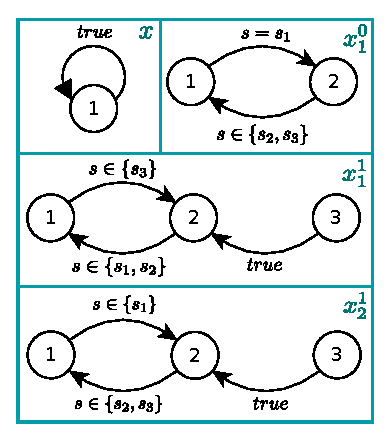
\includegraphics[width=0.7\linewidth]{pic/xupdate2}
%	\caption{ Transition graph of internal variables. Compared to the graph in Figure \ref{fig:eg1}, transition conditions on most edges are different. {\color{purple} What is the difference between the update rule and the transition conditions? I think there is space to put both transition graphs (before and after) on this figure. It would make it easier to see what changed.}}
%	\label{fig:xupdate2}
%\end{figure}

Let the system starts from $ s_1 $ and initialize internal variables as $ (1,1,1,1) $. Only one trajectory is available under control of $\widehat{\mathcal{C}} $, i.e. $ s_1,s_2,s_3,s_2,s_1,...$, where the sequence of actions is $ b,f,g,c,... $ according to the controller execution rules in Definition \ref{def:exec}. The trajectory doesn't visit $ s_4 $, for the system isn't able to jump to $ A $ from $ s_4 $ after action $ e $ is removed.

\subsection{Case study: 1D Hopping Robot}

\begin{figure}
	\centering
	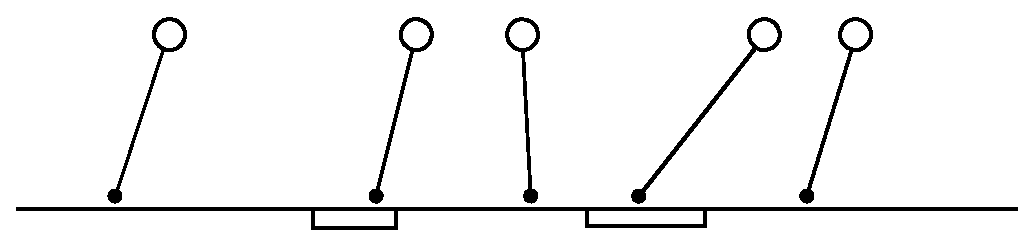
\includegraphics[width=0.8\linewidth]{pic/hop_rob}
	\caption{Hopping robots with point foot on a ground with holes.}
	\label{fig:hoprob}
\end{figure}


Consider a hopping robot moving in a straight line. The robot model is approximated by  Linear Inverted Pendulum Model (LIPM) as follows:
\begin{align}
\begin{bmatrix}
\dot{x}\\
\dot{v}
\end{bmatrix} = \begin{bmatrix}
0 & 1\\
g/h_0 & 0
\end{bmatrix}\begin{bmatrix}
x\\
v
\end{bmatrix}+\begin{bmatrix}
0\\-g/h_0
\end{bmatrix} u \label{eqn: model}
\end{align}
where $x$ is the center of mass (CoM) of the robot; $v$ is the velocity of CoM and $ u $ is position that the robot foot will step on. 

The state space $ Q = [-2.5,2.5]\times [-4,4] $ with action space $ U = [-3.5,3.5] $. Discretize $ Q $ and $ U $ uniformly with grid size $ 0.1 $ and $ 0.2 $, and compute the transitions between discretized grids over-approximately  using the method described in \cite{Liu2014,Sun2014}. Finally we get a AFTS with states indexed $ [1:4000] $, actions $ [1:35] $ and $ 187594 $ valid transitions, which is the abstraction of the hopping robot. 

The specification for the control synthesis is 
\begin{align}
\Diamond \Square B
\end{align}
where $ B=[-2.5,2.5]\times[-2,2] $. It says that the CoM of the robot should always stay within $ [-2.5,2.5] $ with velocity lower than $ 2 $ after finite time from beginning. Given the specification, the winning set and controller are computed via \eqref{win_phi} (taking $ A = Q,B=B , C^1 = Q $).

Now imagine that some holes on the ground are detected, as shown in Figure \ref{fig:hoprob}, where the robot should avoid stepping. Therefore some actions need to be disabled. Once we determine which actions will be affected, we can put them in $ U_d $ and patch the existing controllers for the new action profiles.
\begin{table}
	\caption{Comparison of re-synthesis time and patching time under multiple action profiles. The first row is the set of available actions. The second row is the percentage of transitions left after $ U_d $ is disabled. The last two rows are the time used for re-synthesizing and patching.}
	\begin{tabular}{lllllll}
		\hline 
		$ U_d $ & $ [1] $ &$ [1:5] $ & $ [1:10] $ & $ [1:15] $ & $ [1:20] $ & $ [1:25] $ \\ 
		\hline 
		$ \exists $trans & $ 100\% $ & $ 96.57\% $ & $ 81.22\% $ & $ 60.55\% $ & $ 39.67\% $ & $ 19.00\% $\\
		$ t_{syn}(s) $ & $ 244.2 $ & $ 581.2 $ & $ 756.1 $ & $ 532.7 $ & $ 315.1 $ & $ 129.4 $ \\
		$ t_{pat}(s)$ & $ 3.4 $ & $ 12.6 $ & $ 13.4 $ & $ 13.1 $ & $ 11.4 $ & $ 9.9 $ \\ 
		\hline 
	\end{tabular} 
	\label{tab: exper}
\end{table}

\begin{table}
	\caption{Comparison of re-synthesis time and patching time under random action profiles. The first row is number of unavailable actions ($ \sharp U_d $). For each number, choose 10 random sets of unavailable actions. The last two rows are the average time used for re-synthesizing and patching.}
	\begin{tabular}{ccccccc}
		\hline 
		$ \sharp U_d $ & $ 1 $ &$ 5 $ & $ 10 $ & $ 15 $ & $ 20 $ & $ 25 $ \\ 
		\hline 
		$ t_{syn}(s) $ & $ 289.7 $ & $ 281.1 $ & $ 292.8 $ & $ 358.6 $ &  $ 367.1 $ & $ 618.1 $ \\
		$ t_{pat}(s)$ & $ 3.2 $ & $ 4.1 $ & $ 5.1 $ & $ 7.2 $ & $ 8.3 $ & $ 17.4 $ \\ 
		\hline 
	\end{tabular} 
	\label{tab: exper2}
\end{table}

\begin{figure}
	\centering
	\begin{subfigure}[b]{0.235\textwidth}
		\centering
		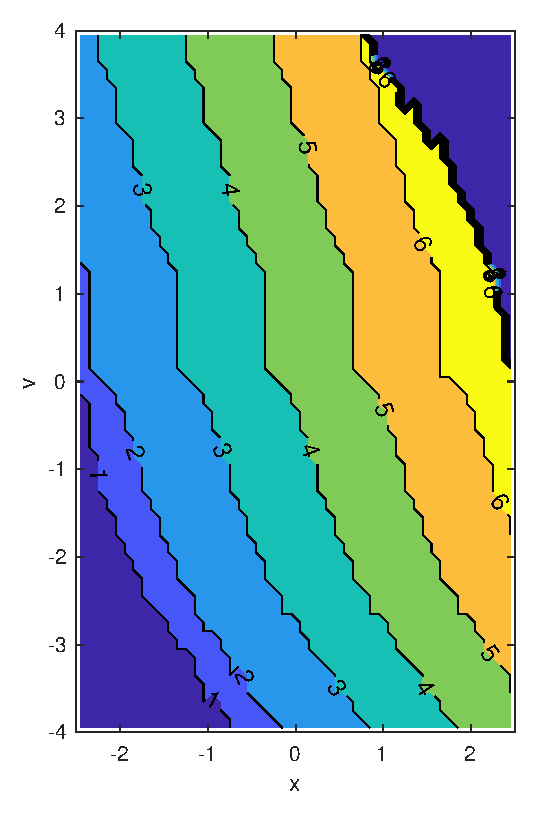
\includegraphics[width=0.8\textwidth]{pic/win_set}
		\caption{winning set}
		\label{fig:win_set}
	\end{subfigure}
	%add desired spacing between images, e. g. ~, \quad, \qquad, \hfill etc. 
	%(or a blank line to force the subfigure onto a new line)
	\begin{subfigure}[b]{0.235\textwidth}
		\centering
		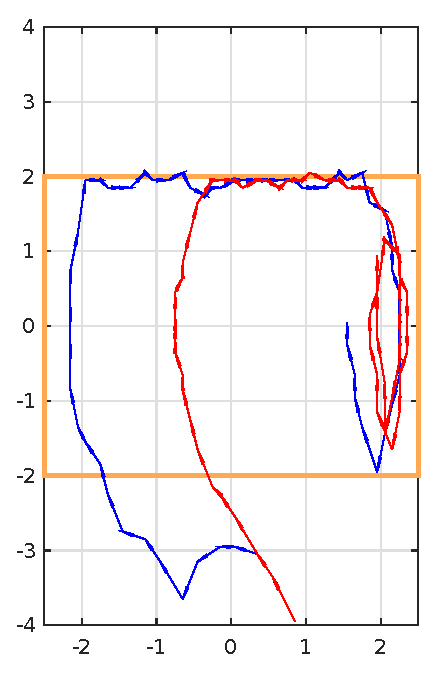
\includegraphics[width=0.8\textwidth]{pic/traj}
		\caption{trajectories}
		\label{fig:traj}
	\end{subfigure}
	%add desired spacing between images, e. g. ~, \quad, \qquad, \hfill etc. 
	%(or a blank line to force the subfigure onto a new line)
	\begin{subfigure}[b]{0.5\textwidth}
		
		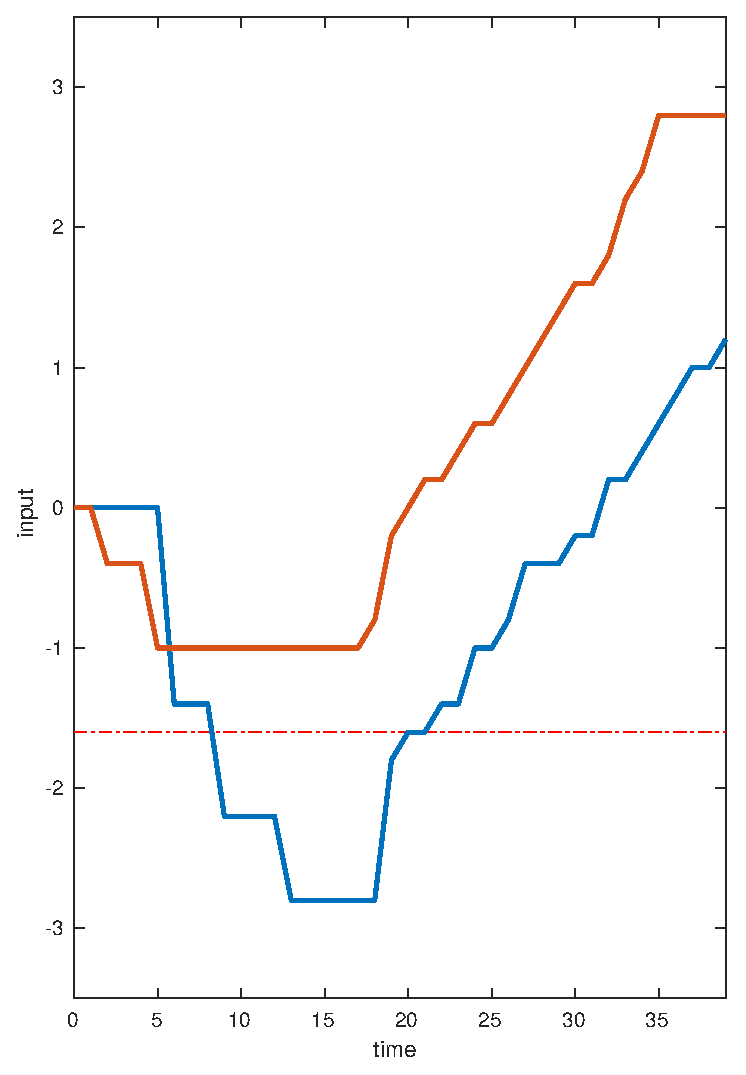
\includegraphics[width=0.9\textwidth]{pic/input}
		\caption{inputs}
		\label{fig:input}
	\end{subfigure}
	\caption{(a) Six regions with different colors are labeled as $ W_1,W_2,...,W6 $. The winning sets under action profiles $U_d = [1], [1:5],[1:10],...,[1:25]$ are represented by $ \bigcup_{i=1}^6 W_i,\ \bigcup_{i=2}^6 W_i,...,\ W_6 $ respectively. (b) Trajectories with initial state $ (0.85,-3.95) $ under $ U_d = \emptyset $ (blue) and $[1:10] $ (red). The region inside orange box is the target set $ B $ (c) Inputs over time under $ U_d = \emptyset $ (blue) and $ [1:10] $ (red) for trajectories in (b). The red dash point line indicates value corresponding to input $ u = 10 $.} %{\color{purple} (a) is a bit hard to understand: we  see only disjoint regions on the image but the winning sets are decreasing in size. Maybe say that the winning set $i$ is the union of the $i$ first regions on the graph. (and redefine them accordingly)}
\end{figure}

The experiment environment is MATLAB R2017a with CPU Intel Core  i7-6820 HQ.

We choose unavailable actions $ U_d= [1],[1:5],...,[1:25] $ for the hopping robot abstraction and compute the controllers via fixed-point operator \eqref{win_phi} and the patching operater \eqref{patching_final} respectively.  The experiment results in Table \ref{tab: exper} make a comparison between the time of synthesizing from scratch ($ t_{syn} $) with the time of patching existing controllers ($ t_{pat} $), which shows that our patching methods can shorten the synthesis time significantly. Figure \ref{fig:win_set} shows the winning sets for each $ U_d $, which shrink to the right part in the state space as $ U_d $ (region of holes) grows.

Furthermore, to show the time efficiency, we randomly choose $ U_d $ with size $n = 1,5,...,25 $, and synthesize the controllers for each $ U_d $ via \eqref{win_phi} and \eqref{patching_final}, and then compare the average time used by the two algorithms for each $ n $, shown in Table \ref{tab: exper2}. The time for our patching algorithm is less than $ 3\% $ of the time for re-synthesizing on average.

Finally, to show that formal guarantees are satisfied after patching, simulation are run for controllers before and after patching for $ U_d =[1:10]$. The initial state is $ s_0=34 $. Figure \ref{fig:traj} and \ref{fig:input} show the trajectories and the inputs used within $ 60 $ time steps. Both trajectories goes into our target region $ B $, indicated by the orange box. The outputs from patched controller is always above the dash line where $ u=10 $, due to the unavailability of actions $[1:10] $.

For practical applications in robot control, if we have the controller for the case that no constraints exists and know all the possible profiles of actions (all the possible constraints on the surface) for a known environment, the patching algorithm can generate the corresponding controllers for those action profiles very quickly. This is actually the motivation of this work.

\section{CONCLUSION}
In this paper, we proposed a method to do fixed-point based control synthesis by patching the existing controller with a larger action space. The correctness of this method relied on the fact that "nested" structure between fixed-point based controllers with "nested" action profiles, so we could do the control synthesis by simply finding out the redundant part of the existing controller for the new profile and then removing them. It gives us a way to avoid the expensive computation cost of synthesis from scratch. 

We illustrated the efficiency of our method on the example of hopping robot. Given the same specification, the time for patching was only $ 1.4\%-7\% $ of the time for synthesis from scratch. 

{\color{purple} Maybe mention that since in some cases a small change of the action set results in a completely different strategy, we expect that in the worst case, our warm-start method does not bring any speed-up. This is similar to classical warm-up techniques in control: there is no guarantee on the speed-up. And then mention that in future work, although we know that getting formal guarantees on a speed-up in average would be hard (since it highly depends on the type of problem), we wish to conduct a finer study of how much speed-up we can expect to achieve with the proposed warm-up, for instance by studying its effect on "random systems and random specifications}

The current work is to apply this method on the control synthesis of hopping robot on a 2D space. If we force the robot to move in 1D and find a finite set of profiles, this method is able to speed up our synthesis process. Besides, it would be interesting to extend this method for the cases that the specification in \eqref{phi} changes or a set of transitions instead of actions in an AFTS is removed. There is a possibility to do these extension as long as Theorem 1 holds.

\iffalse
\section{Appendix}
\textbf{Proof of \eqref{patch_inv}}:

\begin{proof}
	Assume that $ Y_t $ and $ \mathcal{C}_t $ are the winning set and controller resulting from $ \text{Inv}_{\exists}^{D,G} (\widehat{Z}) $. Here we're going to prove that $ Y_t=\widehat{Y}$. Once we have $ Y_t=\widehat{Y}$, it's easy to check that $ T(\mathcal{C}_t) = T(\widehat{C}) $.
	
	By \eqref{win_inv}, the winning set $ Y $ of $ \text{Inv}_{\exists}^{D,G} (Z) $ is the largest subset of $ (G\cap B) - Z  $ satisfying the convergence condition w.r.t $ Z $, i.e. $ Y \subseteq Pre^{T,D}_{\exists, \forall}(Y\cup Z) $, so is $ Y_t $ w.r.t. $ \widehat{Z} $.
	
	We want to show that $ \widehat{Y} = Y_t$: First, show $ Y_t \subseteq Y_0 $ for $ Y_0 $ in \eqref{patch_inv}. Due to $ Y_t \subseteq G\cap B-\widehat{Z} \subseteq (G\cap B -Z)\cup \Delta Z $, we have $ Y_t\cap (G\cap B-Z)\subseteq Y_t $ and $ Y_t\cup \widehat{Z} \subseteq Y_t\cap (G\cap B-Z)\cup Z$. Then $ Pre^{T,D}_{\exists,\forall}(Y_t\cup \widehat{Z}) \subseteq Pre^{T,D}_{\exists,\forall}(Y_t\cap (G\cap B-Z)\cup Z)$. For $ Y_t \subseteq Pre^{T,D}_{\exists,\forall}(Y_t\cup \widehat{Z})$, we have $ Y_t\cap (G\cap B-Z)\subseteq Pre^{T,D}_{\exists,\forall}(Y_t\cap (G\cap B-Z)\cup Z) $. Therefore $ V= Y_t \cap (G\cap B -Z) $ is one subset of $ G\cap B -Z $ satisfying the convergence condition over $ Z $. For $ V_1 $ and $ V_2 $, two subsets of $ G\cap B-Z $ satisfying convergence condition, $ V_1\cup V_2 $ also satisfies this condition, for $ V_1\cup V_2\subseteq \text{Pre}_{\exists,\forall}(V_1\cup Z)\cup \text{Pre}_{\exists,\forall}(V_2\cup Z)\subseteq \text{Pre}_{\exists,\forall}(V_1\cup V_2\cup Z) $. This implies that $ V \subseteq W_{\text{Inv}} $ (otherwise, $ W_{\text{Inv}} $ could be $ W_{\text{Inv}}\cup V $, since $ W_{\text{Inv}} $ is the largest subset of $ G\cap B-Z $ satisfying the convergence condition over $ Z $.) So $ Y_t = V\cup Y_t\cap \Delta Z \subseteq W_{\text{Inv}}\cup (\Delta Z \cap G\cap B) = Y_0$. 
	
	Next, we want to show that $ Y_t \subseteq Y_{\infty} $. It's equivalent to show that $ \Delta Y_k\cap Y_t = \emptyset $, since $ Y_t\subseteq Y_0 $ and $ Y_k = Y_0 - \bigcup_{i\in \{1,2,...,k\}} \Delta Y_k$. Obviously $ \Delta Y_0\cap (Y_t\cup \widehat{Z}) = \emptyset $. Assume that $ \Delta Y_k \cap (Y_t\cup \widehat{Z}) = \emptyset $, then $ \text{Pre}_{\exists,\forall}^{T,D} (Y_t\cup \widehat{Z}) \cap \text{Pre}_{\forall, \exists}^{T_{\text{Inv}}^k,D}(\Delta Y_k) = \emptyset$ by definition of $ Pre $ in \eqref{eqn:pre} and the fact that $ \rightarrow_{T_{\text{Inv}}^k}\subseteq \rightarrow_{T} $. For $ Y_t \subseteq \text{Pre}_{\exists,\forall}^{T,D} (Y_t\cup \widehat{Z}) $ and $ \Delta Y_{k+1} = \text{Pre}_{\forall, \exists}^{T_{\text{Inv}}^k,D}(\Delta Y_k) $, $ Y_t\cap \Delta Y_{k+1} = \emptyset $. Hence by induction argument, $ Y_t \cap \Delta Y_k = \emptyset, \forall k $. Thus, $ Y_t\subseteq Y_{\infty} $. 
	
	The last step is to show that $ Y_{\infty} $ satisfies the convergence condition over $ \widehat{Z} $. By definitions of $ T_{\text{Inv}}^k $, $ \Delta Y_{k+1}= Y_k \cap \text{Pre}_{\forall,\exists}^{T, D}(\Delta Y_k)$. Then by the additivity of $ \text{Pre}^{T,D}_{\forall,\exists} $ (i.e. for any $ X_1 $ and $ X_2 $, $ \text{Pre}_{\forall,\exists}^{T,D} (X_1\cup X_2)=\text{Pre}_{\forall,\exists}^{T,D} (X_1)\cup \text{Pre}_{\forall,\exists}^{T,D} (X_2) $), it's easy to check that redefining fourth line in \eqref{patch_inv} by $ \Delta Y_{k+1} = \Delta Y_k \cup (Y_k \cap \text{Pre}_{\forall,\exists}^{T, D}(\Delta Y_k)) $ gives the same result.  By the new definition of $ \Delta Y_k $ and the fact $ Y_k \cap \widehat{Z} = \emptyset $, $ \Delta Y_k = Q-(Y_k\cup \widehat{Z}) $. $ \Delta Y_k $ converges surely since it increases each iteration and is contained by a finite set $ Q $. Once $ \Delta Y_k $ converges, $ Y_k \cap \text{Pre}_{\forall,\exists}^{T, D}(\Delta Y_k)\subseteq \Delta Y_k $. $ Y_k $ and $ \Delta Y_k $ are disjoint, so $ Y_k \cap \text{Pre}_{\forall,\exists}^{T, D}(\Delta Y_k) = \emptyset $, i.e.  $ Y_k \cap \text{Pre}_{\forall,\exists}^{T, D}(Q-(Y_k\cup \widehat{Z})) = \emptyset $. It says that $ \forall s_1 \in Y_k$, not $\forall u\in D, \exists s_2\in Q, (s1,u,s2)\in \rightarrow_{T} $ and $s_2\in (Q-(Y_k\cup \widehat{Z}))$, i.e. $ \forall s_1 \in Y_k, \exists u\in D, \forall s_2 \in Q,  (s_1,u,s_2)\not\in \rightarrow_{T}$ or $ s_2\in (Y_k\cup \widehat{Z})$. That implies that $ Y_k\subseteq \text{Pre}_{\exists,\forall}^{T,D}(Y_k\cup \widehat{Z}) $. Therefore $ Y_{\infty}\subseteq Y_t $ following the same arguments in step one.
\end{proof}
\fi

%\nocite{*}
\bibliographystyle{eptcs}
\bibliography{warmstart}

\appendix
\section{Fixed-point Operators}\label{app:basic-alg}

In this appendix, we present algorithms from \cite{Nilsson2017} to compute the winning set for a specification in the form \eqref{phi}. In addition to the winning set, these algorithms provide an explicit construction of the control implementation as in Definition \ref{def:cont}. 

The most general algorithm that computes the winning set and the controller for specifications in the form of \eqref{phi} is given in \eqref{win-phi}. The winning set that results from \eqref{win-phi} is equal to $ V_{\infty} $, i.e. the limit of the expanding sequence $V_k$. $ \mathcal{C} $ is the controller corresponding to the winning set $ V_{\infty} $. 

The building blocks for algorithm \eqref{win-phi} are (fixed-point based) operators \eqref{win-interm}, \eqref{win-until}, \eqref{win-pgpre},\eqref{win-inv} and \eqref{eqn:pre}. Each operator corresponds to a type of LTL formula used in \eqref{win-phi}. Note that when a fixed-point operator appears as part of a formula, it only refers to its first output, i.e. the winning set.




\begin{table}
\footnotesize
\begin{tabular}{ll}
	\begin{minipage}{0.5\textwidth}
		\begin{align}
		[V_{\infty},\mathcal{C}] =\  \text{Win}_{\exists, \forall}^{T}\left(\Square A \wedge \Diamond \Square B \wedge \left( \bigwedge_{i\in I} \Square \Diamond R^i\right)\right)\nonumber\\
		=\begin{cases}V_{\text{inv}} = \text{\text{Win}}^{T}_{\exists, \forall} ((A\mathbf{U}\emptyset)\vee \Square (A\wedge \Diamond Q))\\
		\text{Restrict~ synthesis~ to~ }V_{\text{inv}}\\
		V_0 = \emptyset,\ \mathcal{V}=\{\},\ \mathcal{K} = \{\},\  {\color{black} k=0}\\
		%{\color{purple} remove:} while\ V_{k+1} \not= V_k:\\
		{\color{black} repeat:}\\
		\ \ \ \ Z_{k+1} = \text{Pre}_{\exists,\forall}^{T,U} (V_k) \bigcup \text{PGPre}_{\exists,\forall}^{T} (V_k, Q)\\
		\ \ \ \ [V_{k+1}, \mathcal{C}_{k+1}]=\\\ \ \ \ \text{Win}_{\exists,\forall}^{T} ((B \mathbf{\ U\ }Z_{k+1}) \vee \Square (B\wedge ( \bigwedge_{i\in I}\Diamond R^i)))\\
		\ \ \ \ \mathcal{V}(k+1)=V_{k+1},\ \mathcal{K}(k+1) = \mathcal{C}_{k+1}\\
		\ \ \ \ {\color{black} k=k+1}\\
		{\color{black} until \ V_{k} = V_{k-1}}\\
		V_{\infty} = V_k,\ \mathcal{C}=(\mathcal{V},\mathcal{K},x)
		\end{cases}\label{win-phi}
		\end{align}
	\end{minipage}
	\begin{minipage}{0.5\textwidth}
		\begin{align}
		[W_{\infty},\mathcal{C}]= \ \text{Win}_{\exists,\forall}^{T}((B\mathbf{\ U\ }Z)\vee \Square (B\wedge(\bigwedge_{i\in I}\Diamond R^i)) )\nonumber\\
		=\begin{cases}
		W_0 = Q,\ \mathcal{V}=\{\},\ \mathcal{K}=\{\}\\ {\color{black} k=0}\\
		%{\color{purple} remove:} while\ W_{k+1}\not= W_k:\\
		{\color{black} repeat:}\\
		\ \ \ \ Z_{k+1}^i = Z\cup (B\cap R^i\cap \text{Pre}_{\exists, \forall}^{T,U}(W_k))\\
		\ \ \ \ [X^i, \mathcal{C}^i]= \text{Win}_{\exists,\forall}^{T} (B\mathbf{\ U\ }Z_{k+1}^i), \forall i \in I\\
		\ \ \ \ W_{k+1} = \bigcap_{i\in I} X^i\\
		\ \ \ \ {\color{black} k=k+1}\\
		{\color{black} until \ W_{k}= W_{k-1} }\\
		\mathcal{V}(1)=W_k,\\ \mathcal{V}(i+1) = B\cap R^i,\ 
		\mathcal{K}(i) = \mathcal{C}^i, \forall i\in I\\
		W_{\infty} = W_k,\ \mathcal{C} = (\mathcal{V},\mathcal{K},x)
		\end{cases}\label{win-interm}
		\end{align}
	\end{minipage} &
\end{tabular} 
\end{table}
\begin{table}
	\footnotesize
	\begin{tabular}{ll}
		\begin{minipage}{.5\textwidth}
			\begin{align}
			[X_{\infty},\mathcal{C}]= \text{Win}_{\exists,\forall}^{T} (B\mathbf{\ U\ }Z)=\quad\quad\quad\quad\quad\quad\ \ \nonumber\\
			\begin{cases}
			X_0 = \emptyset,\ \mathcal{V}=\{\},\ \mathcal{K}=\{\},\ {\color{black} k=0}\\
			%{\color{purple} remove:} while\ X_{k+1}\not= X_k\\
			{\color{black} repeat:}\\
			\ \ \ \ [V^1_k,C^1_k]=
			\text{Pre}_{\exists,\forall}^{T,U}(X_k)\\
			\ \ \ \  [V^2_k,C^2_k]=\text{PGPre}_{\exists,\forall}^{T}(Z\cup(B\cap V^1_k),B)\\
			\ \ \ \ X_{k+1} =Z\cup (B\cap V^1_k)\cup V^2_k\\
			\ \ \ \ \mathcal{V}(2k+1)=V^1_k, \mathcal{V}(2k+2)=V^2_k\\
			\ \ \ \ \mathcal{K}(2k+1)=C^1_k,\ \mathcal{K}(2k+2)=C^2_k\\
			\ \ \ \ {\color{black} k=k+1}\\
			{\color{black} until \ X_{k}= X_{k-1} }\\
			X_{\infty}=X_k,\ \mathcal{C} = (\mathcal{V},\mathcal{K},x)
			\end{cases}\label{win-until}
			\end{align}
		\end{minipage} &
		\begin{minipage}{.5\textwidth}
			\begin{align}
			[Z_{\infty},\mathcal{C}]=\text{PGPre}_{\exists,\forall}^{T} (Z,B)=\quad \ \nonumber\\
			\begin{cases}
			Z_{\infty} = Z,\ \mathcal{V} = \{\},\ \mathcal{K}=\{\}\\ k = 1\\
			for\ D\in 2^U:\\
			\ \ for\ G\in G(D):\\
			\ \ \ \ [V_k,\mathcal{C}_k]=Inv_{\exists}^{D,G}(Z_{\infty},B)\\
			\ \ \ \  Z_{\infty} = Z_{\infty} \cup V_k\\
			\ \ \ \  \mathcal{V}(k)=V_k,\ \mathcal{K}(k)=\mathcal{C}_k\\
			\ \ \ \  {\color{black} k = k+1}\\
			\mathcal{C} = (\mathcal{V},\mathcal{K},x)
			\end{cases}\label{win-pgpre}
			\end{align}
		\end{minipage} 
	\end{tabular} 
\end{table}

\begin{table}
\footnotesize
\begin{tabular}{ll}
	\begin{minipage}{.5\textwidth}
		\begin{align}
	[W,\mathcal{C}]=\text{Pre}_{\exists,\forall}^{T,U}(V)=\quad \quad \quad \quad \quad \quad \quad\quad\quad\quad\quad\nonumber\\
	\begin{cases}
	W = \{q_1\in Q: \exists (u\in U) \forall (q_2\\\quad\quad s.t.\ (q_1, u, q_2) \in \rightarrow_T), q_2\in V\}\\
	D(q)=\{u\in U: \forall (q_2\ s.t.\ (q,u,q_2)),\ q_2\in V\}\\
	\mathcal{C}=\{(q,D(q)):q\in Q,D(q)\not=\emptyset\}
	\end{cases}\label{eqn:pre}
	\end{align}
	\end{minipage}& 
\begin{minipage}{.5\textwidth}
\begin{align} [Y_{\infty},\mathcal{C}]=\text{Inv}_{\exists}^{D,G}(Z,B)=\ \quad \quad \quad \nonumber\\
\begin{cases}Y_0 = (G\cap B) - Z\\
while\ Y_{k+1}\not=Y_k:\\
\quad Y_{k+1} = Y_k\cap \text{Pre}_{\exists,\forall}^{T,D}(Y_k\cup Z)\\
[-,\mathcal{C}] = Pre^{T,D}_{\exists,\forall}(Y_k\cup Z)\\
Y_{\infty} = Y_k,\ \mathcal{C}\ restricted\ to\ Y_{\infty}
\end{cases} \label{win-inv} \end{align}
\end{minipage} 
\end{tabular} 
\end{table}

\iffalse	
\begin{algorithm}
	\small
	\caption{$ \text{PGPre}_{\exists,\forall}^{T} (Z,B) $}
	\label{alg:algorithm-label}
	\begin{algorithmic}
		\REQUIRE $ T, U, Z, B $\\
		\STATE $ Z_{\infty} = Z,\ \mathcal{V} = \{\},\ \mathcal{K}=\{\}, k = 1 $
		\FOR{$ U\in 2^U $} \FOR{$ G\in G(U) $}
		\STATE $ [V_k,\mathcal{C}_k]=Inv_{\exists}^{U,G}(Z_{\infty},B) $, $ Z_{\infty} = Z_{\infty} \cup V_k $, $ \mathcal{V}(k)=V_k,\ \mathcal{K}(k)=\mathcal{C}_k $, $ {\color{black} k = k+1} $
		\ENDFOR
		\ENDFOR
		\RETURN $ \mathcal{C} = (\mathcal{V},\mathcal{K},x) $
	\end{algorithmic}
	\label{alg: win-pgpre}
	\end{algorithm}
\fi

The winning sets {\color{black} resulting from} \eqref{win-interm}, \eqref{win-until}, \eqref{win-inv} are $ W_{\infty} $, $ X_{\infty} $ and $ Y_{\infty} $. {\color{black} $\text{Pre}_{\exists,\forall}^{T,U}$ is a one-step reachability operator, and $\text{Inv}_{\exists}^{U,G}(Z,B)$ computes $Y_\infty \subseteq (G\cap B) - Z$ from where the state can be controlled (with actions in $U$) to either remain inside $Y_\infty$ or reach $Z$, but because $G$ is a progress group under $U$, remaining indefinitely in $G$ is impossible and therefore $Z$ is
	eventually reached, which is why $Y_\infty$ is a winning set for $B\mathbf{\ U\ }Z$.}
    
    For \eqref{win-phi}, \eqref{win-interm}, \eqref{win-until} and \eqref{win-inv}, the number of sub-controllers in each controller is proportional 
    {\color{purple} the number of children controllers is equal} 
    to the number of iterations before the corresponding fixed-point operator converges. Simple controllers are smallest elements in a controller, i.e. the ones given by \eqref{eqn:pre} and \eqref{win-inv}. 
    
    \section{Proof of Theorem 4}\label{app:pr-31}
    
    {\color{red} Requires careful reading}

\emph{Proof:} Assume that $ Y_t $ and $ \mathcal{C}_t $ are the winning set and the controller resulting from $ \text{Inv}_{\exists}^{D,G} (\widehat{Z}) $. We want to show that $ Y_t=\widehat{Y}$, which immediately implies $ T(\mathcal{C}_t) = T(\widehat{C}) $. {\color{red} is $T$ still defined?}
	
The winning set $ Y $ of $ \text{Inv}_{\exists}^{D,G} (Z) $ is the largest subset of $ (G\cap B) - Z  $ satisfying the convergence condition w.r.t $ Z $, i.e. $ Y \subseteq Pre^{T,D}_{\exists, \forall}(Y\cup Z) $ and $Y$ is the greatest fixed-point of this operator, so is $ Y_t $ w.r.t. $ \widehat{Z} $. Also, $ Y_t \subseteq Y_0 $ for $ Y_0 $ in \eqref{patch-inv} by Theorem \ref{thm: inv-set}. 
	
	First, we show $ Y_t \subseteq \widehat{Y} $: Since $ Y_t\subseteq Y_0 $ and $ Y_k = Y_0 - \bigcup_{i\leq k} \Delta Y_i$, it is enough to show $ \Delta Y_k\cap Y_t = \emptyset,\forall k $. Proceeding by induction: $ \Delta Y_0\cap (Y_t\cup \widehat{Z}) = \emptyset $. Assume that $ \Delta Y_k \cap (Y_t\cup \widehat{Z}) = \emptyset $, then it can be easily checked that $\text{Pre}_{\forall, \exists}^{T_k,D}(\Delta Y_k) \cap  \text{Pre}_{\exists,\forall}^{T,D} (Y_t\cup \widehat{Z}) = \emptyset$ based on the fact that	 $ \rightarrow_{T_k}\subseteq \rightarrow_{T} $. For $ Y_t \subseteq \text{Pre}_{\exists,\forall}^{T,D} (Y_t\cup \widehat{Z}) $ and $ \Delta Y_{k+1} = \text{Pre}_{\forall, \exists}^{T_k,D}(\Delta Y_k) $, $ Y_t\cap \Delta Y_{k+1} = \emptyset $. Hence by induction argument, $ Y_t \cap \Delta Y_k = \emptyset, \forall k $, i.e. $ Y_t\subseteq \widehat{Y} $. 
	
Second, we show $ \widehat{Y}\subseteq Y_t $: It is enough to show that $ \widehat{Y} $ satisfies the convergence condition over $ \widehat{Z} $. By definitions of $ T_k $, $ \Delta Y_{k+1}= Y_k \cap \text{Pre}_{\forall,\exists}^{T, D}(\Delta Y_k)$. Then by the additivity of $ \text{Pre}^{T,D}_{\forall,\exists} $ (i.e. for any $ X_1 $ and $ X_2 $, $ \text{Pre}_{\forall,\exists}^{T,D} (X_1\cup X_2)=\text{Pre}_{\forall,\exists}^{T,D} (X_1)\cup \text{Pre}_{\forall,\exists}^{T,D} (X_2) $), it's easy to see that redefining $ \Delta Y_{k+1} $ in \eqref{patch-inv} by $ \Delta Y_{k+1} = \Delta Y_k \cup (Y_k \cap \text{Pre}_{\forall,\exists}^{T, D}(\Delta Y_k)) $ doesn't change $ Y_{k+1} $.  Based on the new definition of $ \Delta Y_k $ and $ Y_k \cap \widehat{Z} = \emptyset $, we have $ \Delta Y_k = Q-(Y_k\cup \widehat{Z}) $. The limit of redefined $ \Delta Y_k $ exists, for it is increasing and contained by a finite set $ Q $. Once $ \Delta Y_k $ converges, $ Y_k \cap \text{Pre}_{\forall,\exists}^{T, D}(\Delta Y_k)\subseteq \Delta Y_k $. Since $ Y_k=\widehat{Y} $ and $ \Delta Y_k $ are disjoint, $ \widehat{Y} \cap \text{Pre}_{\forall,\exists}^{T, D}(\Delta Y_k) = \emptyset $, i.e.  $ \widehat{Y} \cap \text{Pre}_{\forall,\exists}^{T, D}(Q-(\widehat{Y}\cup \widehat{Z})) = \emptyset $. It says that $ \forall s_1 \in \widehat{Y}$, not $\forall u\in D, \exists s_2\in Q, (s1,u,s2)\in \rightarrow_{T} $ and $s_2\in (Q-(\widehat{Y}\cup \widehat{Z}))$, i.e. $ \forall s_1 \in \widehat{Y}, \exists u\in D, \forall s_2 \in Q,  (s_1,u,s_2)\not\in \rightarrow_{T}$ or $ s_2\in (\widehat{Y}\cup \widehat{Z})$. That implies that $ \widehat{Y}\subseteq \text{Pre}_{\exists,\forall}^{T,D}(\widehat{Y}\cup \widehat{Z}) $, i.e. $ \widehat{Y} $ satisfies the convergence condition over $ \widehat{Z} $. \QEDB
%\end{proof}

\end{document}
